\documentclass[11pt,leqno,oneside]{amsart}
\usepackage[alphabetic,abbrev]{amsrefs} % use AMS ref scheme
\usepackage{../ReAdTeX/readtex-core}
\usepackage{../ReAdTeX/readtex-dangerous}
\usepackage{../ReAdTeX/readtex-abstract-algebra}
\usepackage{../ReAdTeX/readtex-lie-algebras}
\usepackage{./monographs}
\usepackage{caption}
\usepackage{subcaption}
\usepackage{todonotes}
\usepackage{tikz-cd}
\usepackage{tikz}
\numberwithin{thm}{section}

\newcommand{\rootlattice}{\Lambda_R}
\newcommand{\weightlattice}{\Lambda_W}
\newcommand{\T}{T}
\newcommand{\U}{\mathcal{U}}
\renewcommand{\b}{\mathfrak{b}}
\newcommand{\ch}{\operatorname{ch}}
\newcommand{\halfsum}{\rho}
\newcommand{\numposrootcombos}{\mathfrak{P}}

\title[Introduction to the Structure of Semisimple Lie Algebras and
Their Representation Theory]{Introduction to the Structure of Semisimple Lie
Algebras and Their Representation Theory}
\author{George H. Seelinger}
\date{June 2018}
\begin{document}
\maketitle
\section{Introduction}
The representation theory of semisimple Lie algebras is an incredibly
beautiful model of a representation theory, since the simple
representations of semisimple Lie algebras are completely
classified. Furthermore, such a tool is very powerful, since it can be
used to
\begin{itemize}
\item completely classify all simple Lie algebras
\item completely understand the representation theory of simply
  connected Lie groups
\item serve as a guide for understanding the reprsentation theory of
  other algebraic objects
\end{itemize}
In this monograph, we will be more concerned with the former
application and then touch on the general representation theory of
semisimple Lie algebras. \\

Note that, in this monograph, a \emph{linear Lie algebra} is a Lie
algebra that is viewed a subalgebra of \(\gl(V)\), although Ado's
theorem shows that any Lie algebra can be realized in such a
way. Furthermore, a field \(F\) will always be of characteristic \(0\)
and algebraically closed unless otherwise stated.
\section{Weyl's Theorem}
In this section, we seek to prove Weyl's theorem, which provides us
with a characterization of the structure of representations of
semisimple Lie algebras. This section is mostly a rewriting and
expanding of \cite{humph} chapter 6.
\begin{thm}[Weyl's Theorem]\label{weyls-thm}
  Let \(\g\) be a semisimple Lie algebra. If \(\phi \from \g \to
  \gl(V)\) is a representation of \(\g\), then \(\phi\) is completely
  reducible.
\end{thm}
To prove this theorem, we will need to show that, for any
\(\g\)-module \(V\) and any submodule \(W \submodule V\), we get \(V =
W \oplus W'\), where \(W'\) is a complement of \(W\). The easiest way
to do this will be to find some module homomorphism \(f \from V \to
W\) with \(\ker f \intersect W = \{0\}\) and \(W + \ker f = V\). To
construct such a homomorphism, we will need the following.
\begin{defn}
  Let \(\phi \from \g \to \gl(V)\) be a faithful representation of a
  Lie algebra \(\g\) and let \(\beta(x,y) := \tr(\phi(x) \phi(y))\) be
  a bilinear form on \(\g\). Then, for basis \(\{x_1, \ldots, x_n\}\)
  of \(\g\) and \(\{y_1, \ldots, y_n\}\) of \(\g\) such that
  \(\beta(x_i,y_j) = \delta_{ij}\), we define the \de{Casimir element
    of \(\phi\)} to be \[
    c_\phi(\beta) = \sum_i \phi(x_i) \phi(y_i) \in \End(V)
  \]
\end{defn}
\begin{example}
  Let \(\g = \sl_2\) with standard basis \(\{e,h,f\}\). Then, as shown
  in \cite{nilp-las}, we have dual basis \(\{\frac{1}{4}f,\frac{1}{8}h,
  \frac{1}{4}e\}\). Now, if \(\phi\) is the adjoint representation, we get
  \begin{align*}
    c_\phi(\{e,f,h\})
    & = \phi(e)\phi(\frac{1}{4} f) + \phi(h)\phi(\frac{1}{8} h) +
      \phi(f)\phi(\frac{1}{4} e) \\
    & = \frac{1}{4} \ad_e \ad_f + \frac{1}{8} \ad_h^2 + \frac{1}{4}
      \ad f \ad_e \\
    & = \frac{1}{4}(2 e_{1,1} + 2 e_{2,2}) + \frac{1}{8}(4 e_{1,1} + 4
      e_{3,3}) + \frac{1}{4}(2e_{2,2} + 2e_{3,3}) \\
    & = e_{1,1} + e_{2,2} + e_{3,3} \\
    & = Id_3
  \end{align*}
%   However, if we instead take \(\phi\) to be the representation \[
%     \phi(h) = \left(
%       \begin{array}{cc}
%         0&-i\\
%         i&0
%       \end{array}
% \right), \ \ \phi(e) = \frac{1}{2} \left(
%   \begin{array}{cc}
%     1&i\\
%     i&-1
%   \end{array}
% \right), \ \ \phi(f) = \frac{1}{2} \left(
%   \begin{array}{cc}
%     1&-i\\
%     -i&-1
%   \end{array}
% \right)
%   \]
%   we get dual basis \(\{f, \frac{1}{2} h,
%   e\}\) and 
%   \begin{align*}
%     c_\phi(\{e,f,h\})
%     & = \phi(e)\phi(f) + \phi(h)\phi(\frac{1}{2} h) +
%       \phi(f)\phi( e) \\
%     & = \frac{1}{4} \left(
%       \begin{array}{cc}
%         2&-2i \\
%         2i&2
%       \end{array}
% \right) + \frac{1}{2} \left(
%             \begin{array}{cc}
%               1&0\\
%               0&1
%             \end{array}
% \right) + \frac{1}{4} \left(
%                  \begin{array}{cc}
%                    2&2i\\
%                    -2i&2
%                  \end{array}
%                         \right) \\
%     & = Id_2
%   \end{align*}
%   \todo{Something is fishy about this second comutation because the
%     trace of the Casimir element must be 3.}
\end{example}
\begin{lem}
  Take a basis \(\{x_1,\ldots,x_n\}\) of \(\g\) and a basis \(\{y_1,
  \ldots, y_n\}\) of \(\g\) such that, for nondegenerate symmetric
  associative bilinear form \(\beta\) on \(\g\), \(\beta(x_i,y_j)
  = \delta_{ij}\). For \(x \in \g\), if \[ 
    [x,x_i] = \sum_j a_{ij} x_j, \ \ \ [x,y_i] = \sum_j b_{ij} y_j
  \]
  then \(a_{ik} = -b_{ki}\)
\end{lem}
\begin{proof}
  We compute
  \begin{align*}
    a_{ik}
    & = \sum_j a_{ij} \delta_{jk} \\
    & = \sum_j a_{ij} \beta(x_j, y_k) & \text{ by bilinearity}\\
    & = \beta([x,x_i],y_k) \\
    & = \beta(-[x_i,x],y_k)  \\
    & = \beta(x_i, -[x,y_k])  & \text{ by associativity} \\
    & = - \sum_j b_{kj} \beta(x_i, y_j) \\
    & = -b_{ki}
  \end{align*}
\end{proof}
\begin{example}
  Continuing the example above, consider basis \(\{e,h,f\}\) of
  \(\sl_2\) and dual basis with respect to the Killing form,
  \(\{\frac{1}{4}f, \frac{1}{8}h, 
  \frac{1}{4}e\}\). Then, for \(x = ae+bh+cf\), we check that
  \begin{align*}
    [x,e] & = 2be-ch
    & \implies a_{1,1} = 2b, a_{1,2}=-c, a_{1,3} = 0\\
    [x,h] & = -2ae+2cf
    & \implies a_{2,1} = -2a, a_{2,2} = 0, a_{2,3} = 2c\\
    [x,f] & = ah-2bf
    & \implies a_{3,1} = 0, a_{3,2} = a, a_{3,3} = -2b\\
    [x,\frac{1}{4}f]
          & = -\frac{1}{2}bf+\frac{1}{4}ah
    & \implies b_{1,1} = -2b, b_{1,2}=2a, b_{1,3} = 0\\
    [x,\frac{1}{8}h] & = \frac{1}{4}cf-\frac{1}{4}ae
    &\implies b_{2,1} = c, b_{2,2} = 0, b_{2,3} = -a\\
    [x,\frac{1}{4}e] & = -\frac{1}{4}ch + \frac{1}{2}be
    &\implies b_{3,1} = 0, b_{3,2} = -2c, b_{3,3} = 2b
  \end{align*}
\end{example}
\begin{lem}
  For \(x,y,z \in \End(V)\), \[
    [x,yz] = [x,y]z + y[x,z]
  \]
\end{lem}
\begin{proof}
  \begin{align*}
    [x,y]z + y[x,z]
    & = (xy-yx)z + y(xz-zx) \\
    & = xyz - yxz + yxz - yzx \\
    & = xyz - yzx \\
    & = [x,yz]
  \end{align*}
\end{proof}
\begin{prop}
  \(c_\phi(\beta)\) commutes with \(\phi(\g)\) in \(\End(V)\).
\end{prop}
\begin{proof}
  For \(x \in \g\), consider \([\phi(x),c_\phi(\beta)]\). Using the
  lemma immediately above, we get \[
    [\phi(x), c_\phi(\beta)] = \sum_i [\phi(x), \phi(x_i)\phi(y_i)] =
    \sum_i [\phi(x),\phi(x_i)]\phi(y_i) + \phi(x_i)[\phi(x),\phi(y_i)]
  \]
  Moreover, we know that \([\phi(x),\phi(x_i)] = \sum_j a_{ij}
  \phi(x_j)\) and \([\phi(x),\phi(y_i)] = \sum_j b_{ij} \phi(x_j)\),
  with \(a_{ik} = -b_{ki}\) for any \(k\)
  using the same decomposition as in the first of the two
  lemmas. Thus, \[
    [\phi(x), c_\phi(\beta)] = \sum_{i,j} a_{ij} \phi(x_j) \phi(y_i) +
    \sum_{i,j} b_{i,j} \phi(x_i) \phi(y_j) = 0
  \]
\end{proof}
This proposition is vitally important for proving Weyl's theorem. With
this element, we now have an object that must ``behave like a scalar''
with respect to \(\phi(\g)\) in \(\End(V)\). Indeed, in the \(\sl_2\)
example, our Casimir element is exactly the identity, although this
need not always be true:
\begin{prop}
  If \(\phi\) is faithful and irreducible, then \(c_\phi(\beta)\) is a
  scalar in \(\End(V)\).
\end{prop}
\begin{proof}
  Since \(\phi\) is irreducible, we can invoke Schur's Lemma to get
  that \(c_\phi(\beta)\) must be a scalar multiple of the identity map.
\end{proof}
\begin{rmk}
  Note that \(c_\phi(\beta)\) is independent of choice of basis when
  \(\phi\) is faithful, so we will often denote \(c_\phi :=
  c_\phi(\beta)\). For more details, see \cite{humph}*{p 27}.
\end{rmk}
\begin{prop}
  Given Casimir element \(c_\phi\) of faithful representation \(\phi
  \from \g \to \gl(V)\), we get that \[
    \tr(c_\phi) = \dim \g
  \]
\end{prop}
\begin{proof}
  This follows from simply applying the trace operator. \[
    \tr(c_\phi) = \sum_i \tr(\phi(x_i) \phi(y_i)) = \sum_i
    \beta(x_i,y_i) = \dim \g
  \]
\end{proof}
\begin{example}
  The Casimir element of \(\sl_2\) under the adjoint representation
  was precisely \(Id_3\) and \(\tr(Id_3) = 3 = \dim \sl_2\).
\end{example}
\begin{lem}\label{trivial-action-on-codim-1}
  Let \(\phi \from \g \to \gl(V)\) be a representation of a semisimple
  Lie algebra \(\g\). Then, \(\phi(\g) \subset \sl(V)\). 
\end{lem}
\begin{proof}
  We know that, for a semisimple Lie algebra, \([\g,\g] = \g\) by the
  fact that \(\g\) is a direct sum of simple Lie
  algebras. Furthermore, \([\gl(V),\gl(V)] = \sl(V)\) by simple
  computation. Thus, \(\phi(\g) = [\phi(\g), \phi(\g)] \subset
  [\gl(V),\gl(V)] = \sl(V)\). 
\end{proof}
\begin{lem}\label{baby-baby-weyl}
  Let \(\phi \from \g \to \gl(V)\) be a representation of a
  semisimple 
  Lie algebra and let \(W \submodule V\) be irreducible with
  codimension 1. Then, \(\phi\) is completely reducible.
\end{lem}
\begin{proof}
  Without loss of generality, we may assume \(\phi\) is faithful
  \todo{why?}. Now, consider \(c_\phi\) commutes with \(\phi(\g)\), so
  \(c_\phi(g.v) = (c_\phi \circ \phi(g))(v) = (\phi(g) \circ
  c_\phi)(v)\) tells us that \(c_\phi\) is actually a \(\g\)-module
  homormophism on \(V\). Thus, \(c_\phi(W) \subset W\) and \(\ker
  c_\phi\) is a submodule of \(V\). Now, by the lemma above, \(\g\)
  must send all of \(V\) into \(W\) and thus act trivially on the
  quotient module \(V/W\). Therefore, \(c_\phi\) must also act
  trivially since it is simply a linear combination of actions in
  \(\g\). So, it must be that the trace of \(c_\phi\) on \(V/W\) is
  0. However, we know \(\tr_V(c) = \dim \g \neq 0\). Now, since
  \(c_\phi\) acts as a (must be non-zero) scalar on \(W\), it must be
  that \(\ker c_\phi \intersect W = \{0\}\) and \(\ker c_\phi + W =
  V\). Thus, since \(\ker c_\phi\) is a submodule of \(V\), it must be
  that \(\ker c_\phi\) is 1-dimensional and \(V = W \oplus \ker
  c_\phi\). 
\end{proof}
\begin{lem}\label{baby-weyl}
  Let \(\phi \from \g \to \gl(V)\) be a representation of a semisimple
  Lie algebra and let \(W \submodule V\) with codimension 1. Then,
  \(\phi\) is completely reducible. 
\end{lem}
\begin{proof}
  Note that this is the same as the lemma above, but now \(W\) need
  not be irreducible. We will show that we can reduce this lemma to
  the case of the previous lemma \ref{baby-baby-weyl}. By
  \ref{trivial-action-on-codim-1}, 
  we know \(\g\) must act trivially on \(V/W\). Thus, \(V/W \isom F\)
  and we have short exact sequence \[
    0 \to W \to V \to F \to 0
  \]
  Now, if \(\dim W = 1\), \(W\) is irreducible and we can appeal to
  the previous lemma. So, now we proceed by induction and assume the
  result it true for \(\dim W < n\). Let \(\dim W = n\) and \(W\) have
  proper submodule \(W'\). Then, we have short exact sequence \[
    0 \to W/W' \to V/W' \to F \to 0
  \]
  Now, by induction, \(V/W' = W/W' \oplus W''/W'\). However, this
  lifts to a short exact sequence \[
    0 \to W' \to W'' \to F \to 0 
  \]
  However, \(\dim W' < \dim W \implies \dim W'' = \dim W' + 1 < \dim W
  + 1 = \dim V\), so we can apply induction to get a one dimensional
  submodule complementary to \(W'\) in \(W''\), say \(X\), so that
  \(W'' = W' \oplus X\). Thus, we get \[
    V/W' = W/W' \oplus W''/W' = W/W' \oplus (W' \oplus X)/W' \implies
    V = W \oplus X
  \]
  since \(W \intersect X = 0\) and \(\dim W + \dim X = \dim V\). Thus,
  we can repeat this process until we get an irreducible \(W\) and
  appeal to the lemma above (\ref{baby-baby-weyl}) to get the result.
\end{proof}
\begin{proof}[Proof of Weyl's Theorem \ref{weyls-thm}]
  Let \(0 \neq W \propsubgroup V\)  be \(\g\)-modules. Thus, we have
  short exact sequence \[
    0 \to W \to V \to V/W \to 0
  \]
  Let \(U = \{\psi \in \Hom(V,W) \st \exists c \in F, \psi|_W(w) = cw,
  \forall w \in W\}\) and let \(T = \{\psi \in
  \Hom(V,W) \st \psi|_W(w) = 0, \forall w \in W\} \submodule
  U\). Then, we check that \(U\) and \(T\)
  are \(\g\)-submodules of \(\Hom(V,W)\). For \(g \in \g\), \(\psi \in
  U\), and \(w \in W\)
  \begin{align*}
    (g.\psi)(w) & = g.\psi(w) - \psi(g.w) & \text{by the Jacobi
                                            identity} \\
                & = g.(cw) - c(g.w) & \psi \in U \\
                & = c(g.w) - c(g.w) \\
                & = 0
  \end{align*}
  Thus, \(g.\psi|_W = 0\) for all \(g \in \g\). A similar computation
  shows that \(T\) is also a \(\g\)-sucmodule, specifying \(c =
  0\). This also shows that \(\g.U \submodule T\). Now, consider the
  quotient \(U/T\). Every element in \(U/T\) is uniquely determined by
  the scalar \(c\), that is \(\tau \in \psi + T\) if and only if \(\tau|_W =
  \psi|_W = c.1_W\) for scalar \(c\). Thus, we have short exact
  sequence \[
    0 \to T \to U \to F \to 0
  \]
  and thus, by the lemma above (\ref{baby-weyl}), \(U = T \oplus T'\)
  where \(T'\) is a 
  one-dimensional 
  \(\g\)-submodue. If we let \(T' = (\psi),\ \psi \in \End(V,W)\),
  then we can scale \(\psi\) such that \(\psi|_W = 1_W\) since \(\psi
  \not \in T\). Now, since \(\psi\) is a \(\g\)-module homomorphism,
  \(\ker \psi \submodule V\), but \(\ker \psi \neq V\) since \(W
  \intersect \ker \psi = \{0\}\). However, \(\psi\) cannot be injective because \(W
  \propsubgroup V\), which is finite-dimensional, and thus \(\ker \psi
  \neq \{0\}\). Therefore, since \(\psi\) is surjective, we have that
  \(V = W \oplus \ker \psi\) as a non-trivial decomposition of
  \(V\). Thus, we can iteratively continue this process until \(V\)
  has been completely reduced.
\end{proof}
Weyl's theorem has many applications in the representation theory of
semisimple Lie algebras. One immediate consequence is the preservation
of the Jordan decomposition (\cite{humph} section 6.4). That is,
\begin{thm}
  Let \(\g \subset \gl(V)\) be a semisimple linear Lie algebra where
  \(V\) is finite-dimensional. Then, \(\g\) contains the semisimple
  and nilpotent parts in \(\gl(V)\) of all its elements. In
  particular, the abstract and usual Jordan decompositions in \(\g\) coincide.
\end{thm}
\begin{cor}
  Let \(\g\) be a semisimple Lie algebra, \(\phi \from \g \to \gl(V)\)
  a (finite-dimensional) representation of \(\g\). If \(x = s+n\) is
  the abstract Jordan decomposition of \(x \in \g\), then \(\phi(x) =
  \phi(s) + \phi(n)\) is the usual Jordan decomposition of \(\phi(x)\).
\end{cor}
% \begin{example}
%   Consider \(\g = \sl_2\). Then, consider \[
%     h+e = \left(
%       \begin{array}{cc}
%         1&1\\
%         0&-1
%       \end{array}
%     \right)
%   \]
%   Then, \[
%     \ad(h+e) = \left(
%       \begin{array}{ccc}
%         2&-2&0\\
%         0&0&1\\
%         0&0&-2
%       \end{array}
% \right)
%   \]
% \end{example}
\begin{rmk}
  Note that this theorem is a generalization of the following facts.
  \begin{itemize}
  \item A nilpotent \(x \in \g\) is also \(\ad\)-nilpotent.
  \item If \(x \in \g\) is diagonalizable, then \(\ad_x\) is also
    diagonailzable. 
  \end{itemize}
\end{rmk}
We also prove the following, which does not require the theorems
above, but is related to the Jordan decomposition.
\begin{prop}\label{ss-and-nilp-respect-decomp-into-simple-ideals}
  Let \(\g\) be a semisimple Lie algebra, thus decomposing into simple
  ideals \(\g = \g_1 \oplus \cdots \oplus \g_t\). Then, the semisimple
  and nilpotent parts of \(x \in \g\) are the sums of the semisimple
  and nilpotent parts in the various \(\g_i\) of the components of \(x\).
\end{prop}
\begin{proof}
  Take \(x \in \g\), so \(x = x_1 + \cdots + x_t\) with \(x_i \in
  \g_i\) and \(x_i = (x_i)_s + (x_i)_n\). Then, \((\ad_\g (x_i)_s)|_{\g_i} =
  \ad_{\g_i} (x_i)_s\) is a semisimple endomorphism of \(\g_i\) and \((\ad_\g (x_i)_s)|_{\g_j} = 0\) for \(i \neq j\)
  by the direct sum decomposition. Thus, \(\ad_\g (x_i)_s\) is a
  semisimple endomorphism of \(\g\). Now, let \(u = (x_1)_s + \cdots +
  (x_t)_s\). Then, \(\ad_\g u\) is a semisimple endomorphism of \(\g\)
  since \([(x_i)_s, (x_j)_s] = 0\) for all \(i \neq j\). \\

  By a similar argument, if \(v = (x_1)_n + \cdots + (x_t)_n\), then
  \(\ad_\g v\) is a nilpotent endomorphism of \(\g\). Therefore,
  because
  \begin{align*}
    [u,v] & = [(x_1)_s, (x_1)_n] + [(x_1)_s, (x_2)_n] + [(x_2)_n,
            (x_1)_s] + [(x_2)_s, (x_2)_n] + \cdots \\
          & = [(x_1)_s, (x_1)_n] + \cdots + [(x_t)_s, (x_t)_n] \\
          & = 0
  \end{align*}
  Then \(u,v\) are commuting endomorphisms with \(u\) semisimple and
  \(v\) nilpotent, and so by the uniqueness of Jordan decomposition,
  \(x = u+v\) is the Jordan decomposition of \(x\).
\end{proof}
\section{Representations of \(\sl_2(F)\)}
Recall that \(\sl_2(F)\) (where \(F\) is an algebraically closed
field) is the Lie algebra of \(2\) by \(2\)
traceless matrices with standard basis \[
  e = \left(
    \begin{array}{cc}
      0&1\\
      0&0
    \end{array}
\right), \ f = \left(
  \begin{array}{cc}
    0&0\\
    1&0
  \end{array}
\right), \ h = \left(
  \begin{array}{cc}
    1&0\\
    0&-1
  \end{array}
\right)
\]
and relations \[
  [h,e] = 2e, \ [h,f] = -2f, \ [e,f] = h
\]
\begin{prop}
  Let \(V\) be an arbitrary \(\sl_2(F)\)-module. Then, \(h\) acts
  diagonally on \(V\), that is, \(\phi(h)\) is diagonalizable.
\end{prop}
\begin{proof}
  Since \(h\) is semisimple, we get that \(\phi(h)\) is semisimple by
  the corollary above.
\end{proof}
\begin{prop}
  Let \(V\) be an arbitrary \(\sl_2(F)\)-module. Then, \(V\)
  decomposes as a direct sum of eigenspaces. \[
    V = \bigoplus_{\lambda \in F} V_\lambda, \ V_\lambda = \{v \in V \st h.v
    = \lambda v\}
  \]
\end{prop}
\begin{proof}
  Since \(h\) is semisimple, \(\phi(h)\) is semisimple and thus
  diagonalizable, meaning that the set of eigenvectors of \(\phi(h)\)
  forms a basis for \(V\). Thus, we can decompose \(V\) into
  \(\phi(h)\)-eigenspaces. 
\end{proof}
\begin{defn}
  Whenever \(V_\lambda \neq 0\), we call \(\lambda\) a \de{weight} of
  \(h\) in \(V\), and we call \(V_\lambda\) a \de{weight space}.
\end{defn}
\begin{lem}
  Let \(V\) be a finite-dimensional \(\g\)-module. Then, for \(v \in
  V_\lambda\), \(e.v \in V_{\lambda+2}\) and \(f.v \in V_{\lambda-2}\).
\end{lem}
\begin{proof}
  This follows from the following computations:
  \begin{align*}
        h.(e.v) & = [h,e].v + e.h.v & \text{ by the Jacobi identity}
    \\
                & = 2e.v + e.(\lambda v) & \text{ by }\sl_2\text{ relations} \\
                & = (\lambda+2)e.v
  \end{align*}
  Similarly, we get \[
    h.(f.v) = [h,f].v + f.h.v = -2f.v + f.(\lambda v) = (\lambda-2)f.v
  \]
\end{proof}
\begin{prop}
  For finite-dimensional \(\sl_2\)-module \(V\), there exists a
  \(\lambda\) such that \(V_\lambda \neq 0\) but \(V_{\lambda+2} =
  0\). 
\end{prop}
\begin{proof}
  Since \(V\) is finite-dimensional and \(V = \Dunion_{\lambda \in F}
  V_\lambda\) is direct, such a \(\lambda\) must exist.
\end{proof}
\begin{defn}
  A nonzero vector in \(V_\lambda\) annihilated by \(e \in \sl_2\) is
  called a 
  \de{maximal vector of weight \(\lambda\)} or the \de{highest weight
    vector of weight \(\lambda\)}.
\end{defn}
\begin{lem}
  Let \(V\) be an irreducible \(\sl_2(F)\)-module. Let \(v_0\) be a
  maximal vector of weight \(\lambda\) and set \(v_{-1} = 0\) and
  \(v_k = \frac{1}{k!} f^k.v_0\) for \(k \geq
  0\). Then,
  \begin{enumerate}
  \item \(h.v_k = (\lambda - 2k)v_k\)
  \item \(f.v_k = (k+1)v_{k+1}\)
  \item \(e.v_k = (\lambda-k+1)v_{k-1}\)
  \end{enumerate}
\end{lem}
\begin{proof}
  By the previous lemma, \(v_k \in V_{\lambda-2k}\), so \(h.v_k =
  (\lambda-2k)v_k\). \\

  By definition of \(v_k\), \[
    f.v_k = f.\frac{1}{k!} f^k.v_0  = \frac{1}{k!} f^{k+1}.v_0 =
    (k+1)f^{k+1}.v_0 = (k+1)v_{k+1}
  \]
  For the final relation, we use induction on \(k\). When \(k=0\), we
  have \(e.v_0 = 0\) since \(v_0\) is a highest weight vector, and
  thus our formula holds since \(v_{-1} = 0\) by assumption. Now,
  observe
  \begin{align*}
    ke.v_k & = e.f.v_{k-1} & \text{ by part (b), }f.v_j = (j+1)v_{j+1}\\
           & = [e,f].v_{k-1} + f.e.v_{k-1} & \text{ by the Jacobi identity}\\
    & = h.v_{k-1} + f.e.v_{k-1} & \text{ by }\sl_2 \text{ relations}
    \\
           & = (\lambda-2(k-1))v_{k-1} + (\lambda - k +2)f.v_{k-2}
                           & \text{ by part (a) and induction} \\
           & = (\lambda-2k+2)v_{k-1} + (k-1)(\lambda-k+2)v_{k-1}
                           & \text{ by part (b)} \\
           & = k(\lambda-k+1) v_{k-1}
  \end{align*}
  Thus, dividing both sides by \(k\), we get the desired result.
\end{proof}
\begin{prop}
  Let \(V\) be an irreducible \(\sl_2(F)\)-module. Then, for \(m\) the
  smallest integer such that \(v_m \neq 0, v_{m+1} = 0\), we get basis
  \(\{v_0, v_1, \ldots, v_m\}\) for \(V\).
\end{prop}
\begin{proof}
  From formula (a) in the lemma above, it is clear that \(\{v_0,
  \ldots, v_m\}\) are linearly independent since they are eigenvectors
  of different eigenvalues for the \(h\)-action. Furthermore, the
  formulas in the lemma above show us that \(\Span \{v_0, v_1, \ldots,
  v_m\}\) is a non-zero submodule of \(V\). However, since \(V\) is
  irreducible, that must mean that \(V\) is the span of this linearly
  independent set. 
\end{proof}
\begin{prop}
  Let \(V\) be an irreducible \(\sl_2(F)\)-module. Then, given highest
  weight vector \(v\) of weight \(\lambda\), \(\lambda\) must be an
  integer. 
\end{prop}
\begin{proof}
  In the lemma above, take \(k = m+1\) for formula (c). We get, for
  \(v_m \neq 0\) but \(v_{m+1} = 0\), \[
    0 = e.v_{m+1} = (\lambda-(m+1)+1)v_m = (\lambda-m)v_m
  \]
  Thus, it must be that \(\lambda = m \in \Z\).
\end{proof}
\begin{defn}
  We call the weight of a maximal vector \(v_m \in V\), an irreducible
  \(\sl_2(F)\)-module, the \de{highest weight} of \(V\).
\end{defn}
\begin{prop}\label{dim-of-hwt-mod}
  Let \(m\) be the highest weight for irreducible \(\sl_2(F)\)-module
  \(V\). Then, \(\dim V = m+1\) and \(\dim V_\mu = 1\) if \(V_\mu \neq
  0\).
\end{prop}
\begin{proof}
  Given the eigenbasis (relative to the \(h\)-action) \(\{v_0, \ldots,
  v_m\}\), it is immediate that \(\dim V = m+1\). Furthermore, for
  each \(V_\mu \neq 0\), there is a unique eigenvector under the
  \(h\)-action spanning it, up 
  to scalar multiple. Thus,
  \(\dim V_\mu = 1\). 
\end{proof}
To summarize, we have the following theorem.
\begin{thm}\label{sl2-summary}
  Let \(V\) be an irreduclbe \(\sl_2(F)\)-module.
  \begin{enumerate}
  \item Relative to \(h\), \(V\) is a direct sum of weight spaces
    \(V_\mu\) where \(\mu = m, m-2, \ldots, -(m-2), -m\) where \(m+1 =
    \dim V\) and \(\dim V_\mu = 1\) for each \(\mu\).
  \item \(V\) has (up to nonzero scalar multiples) a unique maximal
    vector, whose weight is \(m\).
  \item The action of \(\sl_2(F)\) on \(V\) is given explicitly by the
    formulas in the lemma above, if the basis is chosen
    appropriately. In particular, there exists at most one irreducible
    \(\sl_2(F)\)-module (up to isomorphism) of each possible dimension
    \(m+1\) where \(m \in \Z, m \geq 0\).
  \end{enumerate}
\end{thm}
\begin{proof}
  Part (a) is \ref{dim-of-hwt-mod}. Since \(\dim V = m+1\), we see by
  relations that \(V\) has a highest weight vector of weight \(m\),
  say \(v_m\), and it is unique since its eigenspace, \(V_\mu\), is
  \(1\)-dimensional. Finally, part (c) is just appealing to the lemma above.
  \end{proof}
\begin{cor}
  Let \(V\) be any (finite-dimensional) \(\sl_2(F)\)-module. Then, the
  eigenvalues of \(h\) on \(V\) are all integers, and each occurs
  along with its negative (an equal number of times). Moreover, in any
  description of \(V\) into a direct sum of irreducible submodules,
  the number of summands is precisely \(\dim V_0 + \dim V_1\).
\end{cor}
\begin{proof}
  If \(V = 0\), then the result is immediate. So, given a non-trivial
  \(V\),  Weyl's theorem says \(V\) is completely reducible, so we
  write \(V\) as a direct sum of irreducible submodules. Now, each of
  these irreducible summands must have integer eigenvalues of
  \(h\) and thus, so must \(V\). For the second part of the corollary,
  we note that an irreducible \(\sl_2\)-module must have an occurence
  of a \(0\)-eigenvector or a \(1\)-eigenvector, but it cannot have
  both since the eigenvalues differ by even numbers due to the fact
  that \(h.v_k = (\lambda-2k)v_k\) in the lemma above.
\end{proof}
Let us now explicitly describe these representations, which are easy
to enumerate due to the theorem above.
\begin{example}
  The easiest representation is the trivial one-dimensional
  representation \(\C = V_0\). 
\end{example}
\begin{example}
  Consider \(V = \{e_1,e_2\}\), the ``standard representation'' of
  \(\sl_2\), where \(h.e_1 = e_1\) and \(h.e_2 = -e_2\). Then, \(V = V_{-1}
  \oplus V_1 = \C e_1 \oplus \C e_2\). By the corollary above, this
  representation must be irreducible.
\end{example}
\begin{example}
  Consider \(W = \operatorname{Sym}^2 V\) for \(V\) the standard
  representation above. Then, a basis is given by \(\{e^2, ef,
  f^2\}\) and we have relations
  \begin{align*}
    h.(e \cdot e) & = e \cdot h.e + h.e \cdot e = 2e^2 \\
    h.(e \cdot f) & = e \cdot h.f + h.e \cdot f = 0 \\
    h.(f \cdot f) & = f \cdot h.f + h.f \cdot f = -2 f^2
  \end{align*}
  and so \(W = \C f^2 \oplus \C ef \oplus \C e^2 = V_{-2} \oplus V_0
  \oplus V_2\). Thus, by the corollary above, \(W\) is the irreducible
  representation of dimension 3. Proceeding more generally, one can
  conclude that the irreducible \(\sl_2\)-representation of dimension
  \(n\) is given by \(\operatorname{Sym}^n V\) for \(V\) the standard
  representation by computing \[
    h.(e^{n-k}f^k) = (n-k)\cdot h.e \cdot e^{n-k-1}f^k + k \cdot h.f
    \cdot e^{n-k}f^{k-1} = (n-2k)\cdot e^{n-k} f^k
  \]
\end{example}
\section{Representations of \(\sl_3(F)\)}
In this section, we describe the representations of \(\sl_3(F)\)
following the program in \cite{fulton}. In \(\sl_3(F)\), we do not have a single obvious element to give us an
eigenspace decomposition, in contrast of \(\sl_2(F)\) where the single
element \(h\)
sufficed. Thus, instead, we will consider a 
\(2\)-dimensional subspace of all diagonal matrices in \(\sl_3(F)\),
denoted \(\h \subset \sl_3(F)\). We make use of the fact
\begin{lem}
  Commuting diagonalizable matrices are simultaneously diagonalizable.
\end{lem}
Therefore, we will be able to find simultaneous eigenvectors for the
matrices in \(\h\) that yield an eigenspace decomposition with
eigenvalues \(\alpha \in \h^*\).
\begin{prop}
  Let \(V\) be an arbitrary \(\sl_3(F)\)-module, then \(V\)
  decomposes as a direct sum of eigenspaces \[
    V = \bigoplus_{\alpha \in \h^*} V_\alpha, \ V_\alpha = \{v \in V
    \st h.v = \alpha(h)v, \forall h \in \h\}
  \]
\end{prop}
Thus, looking specifically at \(\sl_3(F)\), we get
\begin{cor}\label{sl3-root-decomp}
  \[\sl_3(F) \isom \h \oplus \left( \bigoplus_{\alpha}
      \g_\alpha \right)\]
  where \(\alpha\) ranges over a finite subset of \(\h^*\) given by
  \(\{\epsilon_i-\epsilon_j \st 1 \leq i,j \leq 3, i \neq j\}\)
  where \[
    \epsilon_i \left(
      \begin{array}{ccc}
        a_1&&\\
           &a_2&\\
        &&a_3
      \end{array}
\right) = a_i
\]
  and, for any \(h \in \h, y \in \g_\alpha\), we get \([h,y] =
  \alpha(h)y\). 
\end{cor}
\begin{proof}
  The decomposition follows from the proposition and the
  finite-dimensionality of \(\sl_3(F)\). To see the specific
  decomposition, let \(D \in \sl_3(F)\) be a diagonal matrix with
  trace \(0\) and let \((m_{i,j}) = M \in \sl_3(F)\). Then, by
  straightforward computation, \[
    [D,M] = \left((a_i - a_j)m_{i,j}\right)
  \]
  and so \([D,M]\) will be a multiple of \(M\) if and only if \(M\)
  has all but one entry equal to \(0\). Thus, \(E_{i,j}\) generate the
  eigenspaces of the adjoint action of \(\h\) on \(\sl_3(F)\), given
  by the \(6\) linear functionals \(\epsilon_i-\epsilon_j\).
\end{proof}
Now, given an \(x \in \g_{\alpha}\), we ask, how does its action
affect this decomposition. We get the following.
\begin{prop}
  Given \(x \in \g_\alpha, y \in \g_\beta\), \([x,y] \in
  \g_{\alpha+\beta}\). In other words, \(\ad(\g_\alpha)\) sends
  vectors in \(\g_\beta\) to \(\g_{\alpha+\beta}\).
\end{prop}
\begin{proof}
  Consider the action of \(\h\) on \([x,y]\).
  \begin{align*}
    [h,[x,y]]
    & = [x,[h,y]] + [[h,x],y]
    & \text{ by the Jacobi identity}\\
    & = [x, \beta(h)y]+[\alpha(h)x,y]
    & \text{ since }y \in \g_\beta, x \in \g_\alpha\\
    & = (\alpha(h)+\beta(h))[x,y]
  \end{align*}
\end{proof}
Later, we will discuss how to visualize this information, but for now
we are content with this understanding. More generally, we see that
\begin{prop}
  Given a representation \(V\) of \(\sl_3\) with eigenspace
  decomposition \(V = \bigoplus_{\alpha} V_\alpha\), then for any \(x
  \in \g_\alpha\) and \(v \in V_\beta\), \(x.v \in
  V_{\alpha+\beta}\). In other words, \(\g_\alpha\) takes \(V_\beta\)
  to \(V_{\alpha+\beta}\).
\end{prop}
From the above situation, we also notice the following
\begin{prop}
  The eigenvalues occurring in an irreducible representation of
  \(\sl_3(F)\) differ by integral linear combinations of the vectors
  \(\{\epsilon_i-\epsilon_j\} \subset \h^*\). 
\end{prop}
\begin{proof}
  Consider
  \begin{align*}
    h.x.v & = x.h.v + [h,x].v
    & \text{ by the Jacobi identity}\\
          & = x.\beta(h)v + \alpha(h)x.v
    & \text{ since } v \in V_\beta, x \in \g_\alpha \\
    & = (\alpha(h)+\beta(h))x.v
  \end{align*}
\end{proof}
Thus, the \(\epsilon_i-\epsilon_j\)'s generate a \emph{lattice} of eigenvalues in \(\h^*\).
\begin{defn}
  The weights of the adjoint representation will be called \de{roots},
  denoted \(\roots\) (this will be expanded on later)
  and the lattice generated by these roots is the \de{root lattice},
  denoted \(\rootlattice\). Furthermore, from the decomposition \(\g =
  \bigoplus_{\alpha \in \h^*} \g_\alpha\) in \ref{sl3-root-decomp},
  the non-zero 
  \(\g_\alpha\)'s will be called \de{root spaces}.
\end{defn}
Now, just as with \(\sl_2(F)\), we wish to find an equivalent notion
to a highest weight
vector for a representation of \(\sl_3(F)\).
\begin{lem}\label{hwtvec-exists}
  Given a representation \(V\) of \(\sl_3(F)\), there exists a \(v \in
  V\) such that
  \begin{enumerate}
  \item \(v\) is an eigenvector for \(\h\)
  \item \(v\) is in the kernel of the action by \(E_{1,2}, E_{1,3}\),
    and \(E_{2,3}\) in \(\sl_3(F)\). (More generally, \(v\) is in the
    kernel of the action of half of the root spaces.)
  \end{enumerate}
\end{lem}
\begin{proof}
  Let us choose linear functional \(\ell \from \h^* \to F\)
  given by \[
    \ell(a_1 \epsilon_1 + a_2 \epsilon_2 + a_3 \epsilon_3) = aa_1 + b
    a_2 + c a_3
  \]
  with \(a+b+c=0\) and \(a>b>c\), such that \(\ell|_{\rootlattice}\) has
  trivial kernel. Thus, we get the equality \[
    \{\g_\alpha \subset \g \st \ell(\alpha) > 0\} =
    \{\g_{\epsilon_1-\epsilon_3}, \g_{\epsilon_2-\epsilon_3},
    \g_{\epsilon_1-\epsilon_2} \}
  \]
  each of which corresponds to a basis matrix with a single nonzero
  entry above the diagonal. Now, pick a \(v \in V_\alpha\) for
  \(\ell(\alpha)\) maximal among the weights of \(V\). Then, each of
  \(E_{1,2}, E_{1,3}\), and \(E_{2,3}\) must kill \(v\) by the
  maximality of \(\alpha\) among the weights with respect to \(\ell\).
\end{proof}
\begin{defn}
  A vector \(v \in V\) that meets the properties of the lemma above is
  a \de{highest weight vector}.
\end{defn}
\begin{prop}
  Let \(V\) be an irreducible \(\sl_3(F)\) representation and \(v \in
  V\) be a highest weight vector. Then, \(V = \langle E_{2,1},
  E_{3,1}, E_{3,2}\rangle.v\), that is, \(V\) is generated by \(v\)
  under successive application of \(E_{2,1}, E_{3,1}\), and \(E_{3,2}\).
\end{prop}
\begin{proof}
  We show that the subspace \(W \subset V\) spanned by images of \(v\)
  under successive application of \(E_{2,1}, E_{3,1}\), and
  \(E_{3,2}\) is preserved by all of \(\sl_3(F)\). Thus, we check
  \begin{align*}
    E_{1,2}.v & = E_{2,3}.v = E_{1,3}.v = 0
    & \text{ by the lemma above} \\
    E_{1,2}.E_{2,1}.v
              & = E_{2,1}.E_{1,2}.v + [E_{1,2},E_{2,1}].v \\
              & = 0 + \alpha([E_{1,2},E_{2,1}])v
    & \text{ since }[E_{1,2},E_{2,1}]\text{ is a diagonal matrix} (\in
      \h) \\
    E_{2,3}.E_{2,1}.v & = E_{2,1}.E_{2,3}.v + [E_{2,3},E_{2,1}].v \\
              & = 0 + 0
                & \text{ since }[E_{2,3},E_{2,1}] = 0
  \end{align*}
  Similar computations hold when applied to
  \(E_{3,2}.v\). Furthermore, since \(E_{1,3} = [E_{1,2},E_{3,2}]\),
  we do not need to check it. \\

  Now, let \(W_n = \Span\{w.v \st w = w_n \cdots w_1, w_i \in
  \{E_{2,1},E_{2,3}\}\}\) (remember that \(E_{3,1} =
  [E_{3,2},E_{2,1}]\)). Then, \(W = \Union_n W_n\). Now, consider that
  \begin{align*}
    E_{1,2}.E_{2,1}.(w_{n-1}\cdots w_1).v
    & = E_{2,1}.E_{1,2}.(w_{n-1} \cdots w_1).v +
      [E_{1,2},E_{2,1}].(w_{n-1} \cdots w_1).v \\
    & \in E_{2,1}.W_{n-2} + \beta([E_{1,2},E_{2,1}]).(w_{n-1}\cdots
      w_1).v & ([E_{1,2},E_{2,1}] \in \h) \\
    & \subset W_{n-1} \\
    E_{2,3}.E_{2,1}.(w_{n-1}\cdots w_1).v
    & = E_{2,1}.E_{2,3}.(w_{n-1}\cdots w_1).v +
      [E_{2,3},E_{2,1}].(w_{n-1}\cdots w_1).v\\
    & \in E_{2,1}.W_{n-2} & ([E_{2,3},E_{2,1}] = 0) \\
    & \subset W_{n-1}
  \end{align*}
  and similarly for applying \(E_{1,2}\) and \(E_{2,3}\) to
  \(E_{3,2}.(w_{n-1} \cdots w_1).v\). Thus, \(W\) is closed under the
  action \(\sl_3(F)\), but \(V\) is irreducible, so \(W = V\).
\end{proof}
In fact, we have slightly more.
\begin{prop}
  Let \(V\) be a \(\sl_3(F)\) representation and \(v \in
  V\) be a highest weight vector. Then, \(\langle E_{2,1}, E_{3,1},
  E_{3,2} \rangle.v\) is an irreducible subrepresentation of \(V\).
\end{prop}
\begin{proof}
  From above, it is clear that \(W := \langle E_{2,1}, E_{3,1},
  E_{3,2} \rangle.v\) is a subrepresentation. Let \(v\) have weight
  \(\alpha \in \h^*\). Then, it must be that \(W_\alpha\) is
  one-dimensional since the action will reduce the weight relative to
  \(\ell\) defined in the proof of \ref{hwtvec-exists}. Assume \(W\) is not
  irreducible, so \(W = W' \oplus W''\). However, the action of \(\h\)
  and projection onto either component commutes, so \(W_\alpha =
  W_{\alpha}' \oplus W_{\alpha}''\). Thus, it must be that either
  \(W_\alpha'\) or \(W_\alpha''\) is zero and so \(v\) either lies in
  \(W'\) or in \(W''\), and thus either \(W = W'\) or \(W = W''\).
\end{proof}
\begin{cor}
  Any irreducible representation of \(\sl_3(F)\) has a unique highest
  weight vector, up to scalar multiple.
\end{cor}
Now, similar to \(\sl_2(F)\), we notice that, given a highest weight
vector, say \(v \in \g_{\epsilon_1-\epsilon_3}\), we have a collection
of vectors \(v, E_{2,1}.v, E_{2,1}^2.v, \ldots\) until \(E_{2,1}^k.v =
0\) for some \(k \in \N\). From this, we note that \(\Span\{E_{2,1},E_{1,2},[E_{1,2},E_{2,1}]\}\) is isomorphic to
\(\sl_2(F)\) via the isomorphism \[
  e \mapsto E_{1,2}, f \mapsto E_{2,1}, h \mapsto [E_{1,2},E_{2,1}]
\]
This leads us to the proposition
\begin{prop}
  The eigenvalues of \(H_{1,2} := [E_{1,2},E_{2,1}]\) on the
  subspace \[
    W = \bigoplus_k V_{\alpha+k(\epsilon_2-\epsilon_1)}
  \]
  are integral and symmetric with respect to \(0\).
\end{prop}
\begin{proof}
  We note that \(W\) is a \(\sl_2(F)\)-representation via the
  isomorphism given above. Thus, since all eigenvalues of
  \(h \in \sl_2(F)\) are integral and symmetric with respect to \(0\)
  for all \(\sl_2(F)\)-representations, that must still be true in
  this case.
\end{proof}
Of course, this process generalizes, and to each root we can
associate a copy of \(\sl_2(F)\).
\section{Beginning of a Structure Theory: Root Space Decomposition}
We now seek to understand the structure of a general semisimple Lie
algebra. 
\begin{defn}
  A subalgebra of a Lie algebra \(\g\) consisting of
  (nonzero) semisimple elements is called a \de{toral subalgebra}
\end{defn}
\begin{lem}
  A toral subalgebra of a Lie algebra \(\g\) is abelian.
\end{lem}
\begin{proof}
  Let \(T\) be a toral subalgebra of \(\g\). We wish to show that
  \([x,T] = 0\) for all \(x \in T\), which is the same as showing
  \(\ad_x = 0\) (where \(\ad\) is taken over \(T\)). Since \(x\) is
  semisimple, so is \(\ad_x\) and 
  since we are working over an algebraically closed field, \(\ad_x\)
  is diagonalizable. Thus, we need only show that all the eigenvalues
  of \(\ad_x\) are \(0\). \\

  Assume that \([x,y] = ay\) for some \(0 \neq a \in F\) and \(y \in
  T\). Then, \(\ad_y x = -ay\) is an eigenvector of \(\ad_y\) with
  eigenvalue \(0\). We may also write \(x\) uniquely as a linear combination of
  eigenvectors of \(\ad_y\), say \(\{-ay, v_1, \ldots, v_{n-1}\}\), since \(y\) is semisimple, \[
    x = -c_0 ay + \sum_{i=1}^{n-1} c_i v_i \implies -ay = \ad_y x = \sum_{i=1}^{n-1}
    c_i \lambda_i v_i
  \]
  where \(\lambda_i\) is the eigenvalue of \(v_i\). However, the set
  \(\{-ay, v_1, \ldots, v_{n-1}\}\) is a basis, so it is linearly
  independent and \(-ay\) cannot be written as a linear combination of
  \(\{v_1, \ldots, v_{n-1}\}\). Thus, we have arrived at a contradiction.
\end{proof}
\begin{defn}
  A toral subalgebra \(\h\) not properly included in any other is called a
  \de{maximal toral subalgebra of \(\g\)}.
\end{defn}
\begin{example}
  Consider \(\g = \sl_2(F)\). Then, \(\h = \langle h \rangle\) is a
  maximal toral subalgebra.
\end{example}
\begin{rmk}
  If \(\g\) is a semisimple Lie algebra, it must have at least one
  element whose semisimple part is nonzero. Otherwise, \(\g\) would be
  nilpotent by Engel's theorem. Thus, \(\g\) contains nonzero toral
  subalgebras and thus contains nonzero maximal toral subalgebras.
\end{rmk}
\begin{defn}
  Let \(\h\) be a maximal toral subalgebra for semisimple Lie algebra
  \(\g\). Then, for \(\alpha \in \h^*\), we define \[
    \g_\alpha := \{g \in \g \st [h,g] = \alpha(h)g, \forall h \in \h\}
  \]
\end{defn}
\begin{defn}
  Let \(\h\) be a maximal toral subalgebra for semisimple Lie algebra
  \(\g\). Then, we define the \de{roots of \(\g\) relative to \(\h\)}
  to be \[
    \roots := \{\alpha \in \h^* \st \g_\alpha \neq 0\}
  \]
\end{defn}
\begin{thm}
  A semisimple Lie algebra \(\g\) admits a decomposition \[
    \g = C_\g(\h) \oplus \bigoplus_{\alpha \in \roots} \g_\alpha, \ \
    \g_\alpha = \{g \in \g \st [h,g] = \alpha(h)g, \forall h \in \h\}
  \]
  for any maximal toral subalgebra \(\h\) of \(\g\).
\end{thm}
\begin{example}
  Let \(\g = \sl_2(F)\). The decomposition above corresponds to
  the decomposition of \(\sl_2(F)\) considered as an
  \(\sl_2(F)\)-modules (the \de{regular representation}). Indeed, if
  \(\h = \Span\{h\}\) for standard basis \((e,f,h)\), then \(C_\g(\h)
  = \h\) and \[
    \sl_2(F) \isom \h \oplus \g_{-2} \oplus \g_2
  \]
  where \(\g_2 = \Span\{e\}\) since \([h,e] = 2e\) and \(\g_{-2} =
  \Span\{f\}\). In fact, a similar decomposition is easy to produce
  for \(\g = \sl_n(F)\) with the standard basis construction.
\end{example}
\begin{rmk}
  In the example above, it is relatively straightforward to compute
\(C_\g(\h) = \h\). In fact, this statement ends up being true for all
semisimple Lie algebras. We wish to show this is true. Furthermore, we
end up finding that \(\roots\) completely characterize the structure
of \(\g\). We seek to show that this is true in the remaining parts of
this section.
\end{rmk}
\begin{prop}
  The \(\ad_h\)-eigenvector decomposition defines an \(\h^*\)-grading
  on \(\g\).
\end{prop}
\begin{proof}
  Let \(x \in \g_\alpha\) and \(y \in \g_\beta\) for \(\alpha,\beta
  \in \h^*\). Then, for \(h \in \h\), \[
    \ad_h([x,y]) = [[h,x],y] + [x,[h,y]] = \alpha(h)[x,y] +
    \beta(h)[x,y] = (\alpha+\beta)(h)[x,y]
  \]
  Thus, \([x,y] \in \g_{\alpha+\beta}\).
\end{proof}
\begin{cor}
    If \(x \in \g_\alpha\) for \(0 \neq \alpha \in \h^*\), then \(\ad_x\) is
  nilpotent. 
\end{cor}
\begin{proof}
  For some \(n \in \N\), \(\g_{n \alpha} = 0\), so \(\ad_x^n = 0\)
  using the grading as above.
\end{proof}
\begin{prop}\label{killing-form-orthogonality}
  Given \(\alpha, \beta \in \h^*\) with \(\alpha+\beta \neq 0\), then,
  relative to the Killing form \(\kappa\) of \(\g\), \(\g_\alpha\) is
  orthogonal to \(\g_\beta\).
\end{prop}
\begin{proof}
  Let \(h \in \h\) such that \((\alpha+\beta)(h) \neq 0\). Then, we
  get
  \begin{align*}
    \alpha(h)\kappa(x,y) & = \kappa([h,x],y)\\
                         & = -\kappa([x,h],y)\\
                         & = -\kappa(x, [h,y]) & \text{by the
                                                 associativity of the
                                                 Killing form.}\\
                         & = -\beta(h)\kappa(x,y)
  \end{align*}
  Thus, \((\alpha+\beta)(h)\kappa(x,y) = 0\). (Recall that the Killing
  form is associative follows from the definition of the bracket on \(\gl(V)\).)
\end{proof}
\begin{cor}
  The restriction of the Killing form to \(C_\g(\h)\) is
  nondegenerate. 
\end{cor}
\begin{proof}
  Since \(\g\) is semisimple, then the Killing form on \(\g\) is
  nondegenerate (see \cite{humph}*{\S 5.1} or
  \cite{nilp-las}*{\S 6}). However, by the proposition above, \(C_\g(\h)
  = \g_0\) is orthogonal to all other \(\g_\alpha\)'s with respect to
  the Killing form. Thus, it must be that, for \(z \in \g_0\), \[
    \kappa(z,\g_0) = 0 \implies \kappa(z,\g) = 0 \implies z = 0
  \]
  by the non-degeneracy of the Killing form on \(\g\). Thus, the
  Killing form is non-degenerate on \(\g_0 = C_\g(\h)\).
\end{proof}
\begin{prop}
  Let \(\h\) be a maximal toral subalgebra of \(\g\). Then, \(\h = C_\g(\h)\).
\end{prop}
\begin{proof}
  We present only an outline of the proof given in \cite{humph}*{\S 8.2}.
  \begin{enumerate}
  \item \(C_\g(\h)\) contains the semisimple and nilpotent parts of
    its elements since \(x \in C_\g(\h) \implies \ad_x(\h) = 0\).
  \item All semisimple elements of \(C_\g(\h)\) lie in \(\h\) since
    \(x \in C_\g(\h) \implies \h+Fx\) is toral and \(\h\) is maximal.
  \item The restriction of \(\kappa\) to \(\h\) is nondegenerate by
    the above items since \([x,\h] = 0\) and \(\ad_x\) is nilpotent
    \(\implies \kappa(x,\h) = 0\).
  \item \(C_\g(\h)\) is nilpotent by Engel's theorem since all its
    elements are \(\ad\)-nilpotent. 
  \item \(\h \intersect [C_\g(\h), C_\g(\h)] = 0\) since
    \([\h,C_\g(\h)] = 0 \implies \kappa(\h,[C_g(\h),C_\g(\h)]) = 0\).
  \item \(C_\g(\h)\) is abelian.
  \item \(C_\g(\h) = \h\), otherwise \(C_\g(\h)\) contains a nonzero
    nilpotent element by above.
  \end{enumerate}
\end{proof}
\begin{cor}
  The Killing form restricted to \(\h\) is non-degenerate.
\end{cor}
\begin{proof}
  Define map \(\theta_h \from \h \to \h\) via \[
    \theta_h(k) = \kappa(h,k).
  \]
  Since the Killing for is non-degenerate on \(\h\), the map \(h
  \mapsto \theta_h\) is an isomorphism between \(\h\) and \(\h^*\)
  since the nondegeneracy gives trivial kernel and dimension count
  gives surjectivity.
\end{proof}
Thus, a maximal toral subalgebra (or a Cartan subalgebra) is
\emph{self-centralizing}. Now, we seek to understand the structure of
the roots.
\begin{lem}
  Given \(\alpha \in \roots\) of semisimple Lie algebra \(\g\) (over
  \(\C\)) and \(0
  \neq x \in \g_\alpha\), then \(-\alpha \in \roots\) and there is a
  \(y \in \g_{-\alpha}\) such that \(\{x,y,[x,y]\}\) spans a Lie
  subalgebra of \(\g\) isomorphic to \(\sl_2(\C)\).
\end{lem}
\begin{proof}
  If \(-\alpha \not\in \roots\), then, for all \(\beta \in
  \roots\), \[
    \kappa(\g_\alpha, \g_\beta) = 0 \implies \kappa(\g_\alpha, \g) = 0
  \]
  by the orthogonality in \ref{killing-form-orthogonality},
  contradicting the non-degeneracy of \(\kappa\). \\

  Next, we note that \(\alpha \neq 0\), so there is a \(t \in \h\)
  such that \(\alpha(t) \neq 0\). Thus, for any \(y \in \g_{-\alpha}\), \[
    \kappa(t,[x,y]) = \kappa([t,x],y) = \alpha(t)\kappa(x,y) \neq 0
    \implies [x,y] \neq 0
  \]
  Now, we observe that \([x,y] \in \h = \g_0\) and \(x,y\) are
  simultaneous eigenvectors for \(\ad[x,y]\), since they are for all
  elements of \(\ad \h\). Thus, \(\Span\{x,y,[x,y]\}\) is a Lie
  subalgebra of \(\g\). \\

  Let \(h := [x,y]\) and let \(S\) be our Lie subalgebra. To see that
  \(S\) is isomorphic to
  \(\sl_2\), we first 
  observe that \(\alpha(h) \neq 0\). Assume otherwise. \[
    [h,x] = \alpha(h)x = 0 = -\alpha(h)y = [h,y]
  \]
  thus showing that \(S\) is a solvable Lie subalgebra. Therefore,
  \([S,S]\) would be a nilpotent Lie subalgebra (see \cite{humph}*{Cor 4.1C}
  or \cite{nilp-las}) and so, in particular, \(\ad([x,y])\) is both
  semisimple and nilpotent, thus implying \(\ad[x,y]=0 \implies [x,y]
  \in Z(S) = 0\), which is a contradiction. Thus, it must be that
  \(S\) is a \(3\)-dimensional complex Lie algebra with \([S,S] = S\),
  which immediately implies that \(S \isom \sl_2(\C)\).
\end{proof}
In fact, this will hold over more general fields, which we will show
below, but this method provides quick insight into the guiding idea
behind the representation theory of semisimple Lie algebras:
understanding roots and the representation theory of
\(\sl_2\). Luckily, we already understand the latter from the section
above. \\

More generally, we have the following orthogonality proposition.
\begin{prop}\label{orthogonality-props}
  \cite{humph}*{Prop 8.3} Let \(\roots \subset \h^*\) be as above for semisimple Lie algebra
  \(\g\) over . Then,
  \begin{enumerate}
  \item \(\roots\) spans \(\h^*\).
  \item If \(\alpha \in \roots\), then \(-\alpha \in \roots\).
  \item If \(\alpha \in \roots, x \in \g_\alpha, y \in \g_{-\alpha}\),
    then \([x,y] = \kappa(x,y)t_\alpha\) where \(t_\alpha \in \h^*\)
    is the unique element such that \(\alpha(h) = \kappa(t_\alpha,
    h)\) for all \(h \in \h\).
  \item Let \(\alpha \in \roots\). Then, \([\g_\alpha, \g_{-\alpha}]\)
    is one dimensional, with basis \(t_\alpha\).
  \item \(\alpha(t_\alpha) = \kappa(t_\alpha, t_\alpha) \neq 0\) for
    \(\alpha \in \roots\).
  \item If \(\alpha \in \roots\) and \(x_\alpha\) is any nonzero
    element of \(\g_\alpha\), then there exists \(y_\alpha \in
    L_{-\alpha}\) such that \(x_\alpha, y_\alpha, h_\alpha =
    [x_\alpha, y_\alpha]\) span a three dimensional simple subalgebra
    of \(\g\) isomorphic to \(\sl_2(F)\) via \[
      x_\alpha \mapsto e, y_\alpha \mapsto f, h_\alpha \mapsto h
    \]
  \item \(h_\alpha = \frac{2t_\alpha}{\kappa(t_\alpha, t_\alpha)}\)
    and \(h_\alpha = -h_{-\alpha}\).
  \end{enumerate}
\end{prop}
\begin{rmk}
  This proposition will later show that \(\roots\) satisfies the axioms of a
  ``root system'' and is thus justifies the terminology ``roots of
  \(\g\) relative to \(\h\).''
\end{rmk}
\begin{example}
  Let us demonstrate the result for \(\g = \sl_2(F)\) since we have
  already shown what needs to be shown in the previous section. Then, \(\h = \Span\{h\} \isom F\) and so
  \(\h^* 
  = \Span\{h^*\} \isom F\) where \(h^*(h) = 1, h^*(e) = 0 = h^*(f)\) and
  \(\roots = \{\pm 2 h^*\}\) since \[
    \sl_2 = \h \oplus \g_2 \oplus \g_{-2}
  \]
  In this case, (a) and (b) above are immediate. For (c), we check \[
    \kappa(e,f) = \tr(\ad_e \ad_f) = 4 
  \]
  and \[
    [e,f] = h \implies t_2 = \frac{1}{4} h^*
  \]
  Indeed, one easily checks \(\kappa(\frac{1}{4} h, \lambda h) =
  \lambda \cdot 2\) for all \(\lambda \in F\). \\

  For (d), \([\g_2, \g_{-2}] = \Span\{[e,f]\} = \Span\{h\}\) is one
  dimensional with basis given by \(\frac{1}{4} h\). \\

  For (e), \(2 \cdot \frac{1}{4} h^*(h) = \frac{1}{16} \kappa(h,h) =
  \frac{1}{2}\). \\

  For (f), the result is trivial. For (g), we note \[
    \frac{2 \frac{1}{4} h}{\frac{1}{16}\kappa(h,h)} =
    \frac{\frac{1}{2}h}{\frac{1}{2}} = h
  \]
\end{example}
\begin{proof}
  For (a), assume \(\roots\) does not span \(\h^*\). Then, there is a
  \(0 \neq h \in \h\) such that \(\alpha(h) = 0\) for all \(\alpha \in
  \roots\). However, this gives, for all \(\alpha \in \roots\), \[
    [h,\g_\alpha] = 0 \implies [h,\g] = 0 \iff h \in Z(\g) = 0
  \]
  which is a contradiction. \\

  (b) is already proven in the lemma above. \\

  For (c), take \(\alpha \in \roots, x \in \g_{\alpha}, y \in
  \g_{-\alpha}\). Then, \[
    \kappa(h,[x,y]) = \kappa([h,x],y) = \alpha(h)\kappa(x,y) =
    \kappa(t_\alpha, h)\kappa(x,y) = \kappa(\kappa(x,y)t_\alpha,h) = \kappa(h,\kappa(x,y)t_\alpha)
  \]
  and so, subtracting the two sides, we have
  \([x,y]-\kappa(x,y)t_\alpha\) is perpendicular to all \(h \in
  \h\). However, since \(\kappa\) is non-degenerate, this means that
  \([x,y] - \kappa(x,y)t_\alpha = 0\). \\

  For (d), we see that \(t_\alpha\) spans \([\g_\alpha,
  \g_{-\alpha}]\) assuming \([\g_\alpha, \g_{-\alpha}] \neq 0\) by part
  (c). Thus, we need only show that \([\g_\alpha, \g_{-\alpha}] \neq
  0\). Following the same technique as the proof of the lemma above,
  assume \(\kappa(x, \g_{-\alpha}) = 0\). Then, \(\kappa(x,\g) = 0\)
  is a contradiction since \(\g\) is semisimple. Thus, there is a \(y
  \in \g_{-\alpha}\) such that \(\kappa(x,y) \neq 0 \implies [x,y]
  \neq 0\). \\

  For (e), assuming \(\alpha(t_\alpha) = 0 \implies [t_\alpha, x] = 0
  = [t_\alpha, y]\) for all \(x \in \g_\alpha, y \in
  \g_{-\alpha}\). However, we can find an \(x,y\) such that
  \(\kappa(x,y) \neq 0\) and, multiplying by scalars, we may assume
  \(\kappa(x,y) = 1 \implies [x,y] = t_\alpha\) by (c). Thus, using
  the same line of reasoning in the lemma, if we let \(S =
  \Span\{x,y,t_\alpha\}\), then \(\ad_\g t_\alpha = 0 \implies
  t_\alpha \in Z(S) = 0\), which is a contradiction. \\

  For (f), let \(0 \neq x_\alpha \in \g_\alpha\) and find a \(y_\alpha
  \in \g_{-\alpha}\) such that \[
    \kappa(x_\alpha, y_\alpha) = \frac{2}{\kappa(t_\alpha, t_\alpha)}
  \]
  using (e) and the fact \(\kappa(x_\alpha, \g_{-\alpha}) \neq
  0\). Then, by (c),
  \begin{align*}
    h_\alpha := \frac{2 t_\alpha}{\kappa(t_\alpha, t_\alpha)}
    \implies & [x_\alpha, y_\alpha] = h_\alpha \\
    & [h_\alpha, x_\alpha] = \frac{2}{\alpha(t_\alpha)}[t_\alpha,x_\alpha] =
      \frac{2 \alpha(t_\alpha)}{\alpha(t_\alpha)}x_\alpha = 2 x_\alpha
    \\
    & [h_\alpha, y_\alpha] = -\frac{2}{\alpha(t_\alpha)}[t_\alpha,
      y_\alpha] = -\frac{2 \alpha(t_\alpha)}{\alpha(t_\alpha)}
      y_\alpha = -2 y_\alpha
  \end{align*}
  Thus, \(\{x_\alpha, y_\alpha,h_\alpha\}\) span a three dimensional
  subalgebra of \(\g\) with the \(\sl_2(F)\) relations.\\

  For (g), we note that \(t_\alpha = -t_{-\alpha}\) since
  \(\kappa(-t_{-\alpha}, h) = \alpha(h) = \kappa(t_\alpha, h)\) for
  all \(h \in \h\). Thus, since \(h_\alpha =
  \frac{2t_\alpha}{\kappa(t_\alpha, t_\alpha)}\), \[
    -h_{-\alpha} =
    -\frac{2t_{-\alpha}}{\kappa(t_{-\alpha},t_{-\alpha})} =
    \frac{2t_\alpha}{\kappa(t_\alpha, t_\alpha)} = h_\alpha
  \]
\end{proof}
As noted above, the correspondence of \(\sl_2(F)\) inside any semisimple
Lie algebra to a root is incredibly important, so much so that we will
define a new notation to refer to such a copy of \(\sl_2(F)\).
\begin{defn}
  For a pair of roots \(\alpha, -\alpha\), let \(\sl(\alpha) \isom
  \sl_2(F)\) be a subalgebra of the form presented in the lemma or
  part (f) of the proposition above, that is, a subalgebra generated
  by \(\{x_\alpha, y_\alpha, [x_\alpha,y_\alpha]\}\) for \(x_\alpha
  \in \g_\alpha\) and \(y_\alpha \in \g_{-\alpha}\).
\end{defn}
With this terminology, we have the following proposition
\begin{prop}
  Given a semisimple Lie algebra \(\g\) with root \(\alpha\), \(\g\)
  may be considered as an \(\sl(\alpha)\)-module via the adjoint
  action, that is, for \(a \in \sl(\alpha), g \in \g\) \[
    a.g = \ad_a g = [a,g]
  \]
\end{prop}
\begin{proof}
  This module is simply a restriction of the adjoint representation.
\end{proof}
\begin{defn}
  Let \(\g\) be a semisimple Lie algebra with roots \(\roots\). Let
  \(\beta \in \roots\) or \(\beta = 0\). Then, subspace \[
    \bigoplus_{\substack{k \in F \\ \beta + k \alpha \in \roots}} \g_{\beta + k \alpha}
  \]
  is an \de{\(\alpha\)-root string through \(\beta\)}.
\end{defn}
Note that such a root string is an \(\sl(\alpha)\)-module. Now, using
this notion, we prove the following.
\begin{lem}\label{only-multiples-of-root-are-pm}
  Let \(\roots \subset \h^*\) be a set of roots for a semisimple Lie
  algebra \(\g\). Then, for \(\alpha \in \roots\), the only multiples
  of \(\alpha\) which lie in \(\roots\) are \(\pm
  \alpha\). Furthermore, \(\g_{\alpha}\) is one-dimensional for every
  root \(\alpha \in \roots\).
\end{lem}
\begin{proof}
  Let \[
    M := \h \oplus \bigoplus_{k \alpha \in \roots} \g_{k \alpha}
  \]
  be the \(\alpha\)-root string through \(0\). 
  If \(c \alpha\) is a root, then \(h_\alpha.x_{c\alpha} =
  2c\alpha(h_\alpha)x_{c \alpha} = 2c x_{c \alpha}\), so \(h_\alpha\)
  has \(2c\) as an eigenvalue. However, the eigenvalues of
  \(h_\alpha\) must be integral, so \(2c \in \Z\). Now, by direct
  computation, 
  \(\sl(\alpha)\) acts trivially on \(\ker \alpha \subset \h\). Next,
  given \(\h + \sl(\alpha)\), we know that, as \(\sl(\alpha)\)-modules, \[
    \h + \sl(\alpha) \isom \ker \alpha \oplus \sl(\alpha)
  \]
  since \(\dim \ker \alpha = \dim \h - \dim \im \alpha = \dim \h -
  1\). Thus, by Weyl's theorem and the above computation, \[
    \h + \sl(\alpha) \subset \h \oplus \bigoplus_{k \alpha \in \roots}
    \g_{k \alpha} \isom \ker \alpha \oplus \sl(\alpha) \oplus N
  \]
  where \(N\) is some complementary submodule. Now, let \(V\) be an
  irreducible representation of \(\sl_2(F)\) with dimension
  \(k\). Then, if \(k\) is even, there is a \(v \in V\) with
  \(h_\alpha .v = 0
  \implies \alpha(v) = 0 \implies v \in \ker \alpha\) by virtue of the
  classification of 
  \(\sl_2(F)\) representations. However, \(\ker \alpha \intersect V =
  0 \implies v = 0\), which is a contradiction. Thus, the only even
  weights occuring in \(M\) are \(0\) and \(\pm 2\), which tells us
  that \(2 \alpha\) cannot be a root. However, this also means that
  \(\frac{1}{2} \alpha\) is not a root, so \(1\) also cannot be a
  weight of \(M\). Thus, since the number of irreducible
  \(\sl_2(F)\)-module summands is precisely \(\dim M_0 + \dim M_1\),
  it must be that \(N\) contains no irreducible
  \(\sl_2(F)\)-submodules, and is thus trivial. Therefore, \[
    M \isom \ker \alpha \oplus \sl(\alpha)
  \]
  but \(\ker \alpha \isom \g_0\) can only be a direct sum of trivial
  \(\sl(\alpha)\)-modules by the classification of \(\sl_2(F)\)
  representations. Thus, \(\g_\alpha\) is one-dimensional since 
  \(\sl(\alpha) = \g_\alpha + \g_{-\alpha} + [\g_\alpha, \g_{-\alpha}]\).
\end{proof}
\begin{prop}\label{integrality-props}
  \cite{humph}*{Prop 8.4} Let \(\alpha, \beta \in \roots\) with
  \(\beta \neq \pm 
  \alpha\). Then,
  \begin{enumerate}
  \item \(\beta(h_\alpha) \in \Z\)
  \item There exist integers \(r,q \geq 0\) such that \(\beta + k
    \alpha \in \roots\) if and only if \(k \in \Z\) and \(-r \leq k
    \leq q\). Furthermore, \(\beta(h_\alpha) = r-q\).
  \item \(\beta - \beta(h_\alpha)\alpha \in \roots\)
  \item If \(\alpha+\beta \in \roots\), then \([\g_\alpha,\g_\beta] =
    \g_{\alpha+\beta}\).
   \item \(\g\) is generated (as a Lie algebra) by the root spaces
     \(\g_\alpha\).
  \end{enumerate}
\end{prop}
\begin{proof}
  We will now look at the action of \(\sl(\alpha)\) on \[
    M := \bigoplus_{\substack{k \in \Z \\ \beta+k\alpha \in \roots}}
    \g_{\beta+k\alpha}.
  \] Since \(h_\alpha.w = \beta(h_\alpha)w\) for \(w \in \g_\beta\),
  it must be that \(\beta(h_\alpha) \in \Z\). From the lemma above, 
  there can be no \(k\) such that \(\beta+k\alpha = 0\) since,
  otherwise, \(\beta\) would be a multiple of \(\alpha\). Thus, the
  action of \(h_\alpha\) on each one-dimensional root space is given
  by \[
    h_\alpha.v = (\beta(h_\alpha)+2k)v
  \]
  for \(v \in \g_{\beta+k\alpha}\). Because the weights differ by even
  integers, it cannot be that both \(0\) and \(1\) occur as a weight
  of this form, and either can only appear once. Thus, \(M\) must be
  an irreducible \(\sl(\alpha)\)-module and the weights must be
  symmetric around \(0\). Let the heighest weight be given by
  \(\beta+q\alpha\) and the lowest weight by
  \(\beta-r\alpha\). Thus, \[
    -(\beta(h_\alpha)+2q) = \beta(h_\alpha)-2r \implies
    \beta(h_\alpha) = r-q
  \]
  which also tells us that \[
    \beta - \beta(h_\alpha)\alpha = \beta - (r-q)\alpha \in \roots
  \]
  since \(-r \leq q-r \leq q\).

  Now, for (d), let \(v \in \g_\beta\) and \(\ad_{x_\alpha} x_\beta =
  0\). Then, \(x_\beta\) is a highest weight vector of \(M\) with
  weight \(\beta(h_\alpha)\). However, we also know that if
  \(\alpha+\beta\) is a root, then \(h_\alpha\) acts on
  \(\g_{\alpha+\beta}\) by eigenvalue \((\alpha+\beta)h_\alpha =
  \beta(h_\alpha)+2\), which tells us that \(\beta(h_\alpha)\) is not the
  highest weight, a contradiction. Thus, it must be that
  \(\ad_{x_\alpha} x_\beta \neq 0 \implies [\g_\alpha, \g_\beta] =
  \g_{\alpha+\beta}\).

  Finally, by virtue of (d), \(\g\) is generated as a Lie algebra by
  the root spaces since, given generator \(t_\alpha \in \g_\alpha\)
  and \(t_\beta \in \g_\beta\), if \(\alpha+\beta \in \roots\),
  \([t_\alpha,t_\beta]\) is a non-zero scalar multiple of
  \(t_{\alpha+\beta}\). 
\end{proof}
\begin{defn}
  The integers \(\beta(h_\alpha)\) are called the \de{Cartan integers}.
\end{defn}
At this point, we now understand a lot of the structure constants of
\(\g\) using the basis given by the root space decomposition. Namely,
the action of \(\h\) is determined by the roots,
\([x_\alpha,x_\beta]\) is determined by the roots for \(\beta \neq \pm
\alpha\), and \([x_\alpha, x_{-\alpha}]\) is a scalar multiple of
\(h_\alpha\). Finally, we wish to prove \(\roots\) has a
well-understood strucutre.
\begin{lem}\label{killing-form-on-roots-is-rational}
  If \(\alpha,\beta \in \roots\), then \(\kappa(h_\alpha, h_\beta) \in
  \Z\) and \(\kappa(t_\alpha, t_\beta) \in \Q\).
\end{lem}
\begin{proof}
  We first realize that \[
    \kappa(h_\alpha, h_\beta) = \tr(\ad_{h_\alpha} \ad_{h_\beta}) =
    \sum_{\gamma \in \roots} \gamma(h_\alpha)\gamma(h_\beta)
  \]
  since the trace is the sum of the eigenvalues with
  multiplicity. However, all these eigenvalues are integers, so
  \(\kappa(h_\alpha, h_\beta) \in \Z\). Next, we compute \[
    \kappa(t_\alpha, t_\beta) =
    \kappa \left(\frac{\kappa(t_\alpha,t_\alpha)}{2}h_\alpha,
    \frac{\kappa(t_\beta,t_\beta)}{2} h_\beta \right) =
    \frac{\kappa(t_\alpha, t_\alpha) \kappa(t_\beta,
      t_\beta)}{4}\kappa(h_\alpha, h_\beta)
  \]
  However, \[
    \frac{1}{\kappa(t_\alpha, t_\alpha)} =
    \frac{1}{4}\kappa\left(\frac{2t_\alpha}{\kappa(t_\alpha,
      t_\alpha)},\frac{2t_\alpha}{\kappa(t_\alpha, t_\alpha)}\right) =
  \frac{1}{4}\kappa(h_\alpha,h_\alpha) \in \Q
  \]
  and thus \(\kappa(t_\alpha,t_\beta) \in \Q\) since it is a product
  of rational numbers.
\end{proof}
\begin{defn}
  Let us define form \((\cdot,\cdot) \from \h^* \times \h^* \to F\)
  via \[
    (\gamma, \delta) := \kappa(t_\gamma, t_\delta)
  \]
  for \(\gamma, \delta \in \h^*\)
\end{defn}
\begin{prop}
  Such a form is non-degenerate and bilinear.
\end{prop}
\begin{proof}
  Since the Killing form is non-degenerate on \(\g\), it is
  non-degenerate on \(\h\) and thus \((\cdot, \cdot)\) is
  non-degenerate on \(\h^*\). Furthermore, \((\cdot, \cdot)\) inherits
  its bilinearity from the Killing form. 
\end{proof}
\begin{lem}
  If \(\beta \in \roots\) and \(\{\alpha_1, \ldots, \alpha_n\}\) is a
  basis of roots for \(\h^*\), then \(\beta\) is a rational linear
  combination of the \(\alpha_i\)'s.
\end{lem}
\begin{proof}
  Consider \(\beta = \sum c_i \alpha_i\). Then, we compute \[
    (\beta, \alpha_j) = \sum_i (\alpha_i, \alpha_j)c_i
  \]
  which gives us \(n\) equations with \(n\) unknowns with rational
  coefficients. Since \((\cdot, \cdot)\) is non-degenerate, the
  associated matrix is non-degenerate and thus
  invertible. Furthermore, since all the coefficients are rational,
  its solutions will be rational. Thus, \(c_i \in \Q\).
\end{proof}
\begin{defn}
  Let \(\g\) be a semisimple Lie algebra with roots \(\roots\). Then,
  we define \(E_\Q \subset \h^*\) to be the \(\Q\)-subspace spanned by
  all the roots \(\roots\).
\end{defn}
By virtue of the proposition above, we know that all roots are
\(\Q\)-linear combinations of other roots, so \(E_\Q\) is independent
of choice of roots for a basis. We now wish to show \((\cdot, \cdot)\) has
more structure on \(E_\Q\).
\begin{prop}
  The restriction of \((\cdot,\cdot)\) to
  \(E_\Q\) is rational and positive-definite
\end{prop}
\begin{proof}
  From lemma \ref{killing-form-on-roots-is-rational}, we know that
  \(\kappa(t_\alpha, t_\beta) \in \Q\) 
  for any 
  roots \(\alpha,\beta \in \roots\), but \(\roots\) \(\Q\)-spans \(E_\Q\) by
  the proposition above,
  and so we can pick a basis of roots for \(E_\Q\), say \(\{\alpha_1,
  \ldots, \alpha_n\}\). Thus, for \(\gamma, \delta \in E_\Q\), \[
    (\gamma, \delta) = \left( \sum c_i \alpha_i, \sum d_j \alpha_j
    \right) = \sum_{i,j} c_i d_j \cdot (\alpha_i, \alpha_j) = \sum_{i,j} c_i
    d_j \kappa(t_{\alpha_i},t_{\alpha_j})
  \]
  but \(c_i,d_j \in \Q\) by definition of \(E_\Q\). Finally, given
  \(\lambda \in E_\Q\), \[
    (\lambda, \lambda) = \sum_{\gamma \in \roots} \gamma(t_\lambda)^2
    = \sum_{\gamma \in \roots} (\gamma, \lambda)^2 \geq 0
  \]
  If \((\lambda,\lambda) = 0\), then \(\gamma(t_\lambda) = 0\) for all
  roots \(\gamma\), and so \(\lambda = 0\) by
  \ref{orthogonality-props} (e).
  Thus, \((\cdot, \cdot)\) is positive-definite.
\end{proof}
\begin{lem}\label{eval-is-root-sys-refln}
  \(\beta(h_\alpha) = \frac{2(\beta,\alpha)}{(\alpha,\alpha)}\)
\end{lem}
\begin{proof}
  Using the fact that \(h_\alpha =
  \frac{t_\alpha}{\kappa(t_\alpha,t_\alpha)}\), we see \[
    \frac{2(\beta,\alpha)}{(\alpha,\alpha)} =
    \frac{2\kappa(t_\beta,t_\alpha)}{\kappa(t_\alpha,t_\alpha)} =
    \kappa\left( t_\beta, \frac{2t_\alpha}{\kappa(t_\alpha,t_\alpha)}
    \right) = \kappa(t_\beta, h_\alpha) = \beta(h_\alpha)
  \]
\end{proof}
\begin{defn}
  Let \(E := \R \otimes_\Q E_\Q\).
\end{defn}
\begin{rmk}
  Using standard linear algebra, the form \((\cdot,\cdot)|_{E_\Q}\)
  extends canonically to \(E\) and is still positive-definite. Thus,
  \(E\) is a Euclidean space.
\end{rmk}
Thus, we see that we have already shown \(\roots\) has a incredibly
useful structure:
\begin{prop}\label{roots-form-root-system}
  Given a semisimple Lie algebra \(\g\), \(\roots\) is a \emph{root
    system} in \(E\), that is
  \begin{enumerate}
  \item \(\roots\) spans \(E\) and \(0 \not \in \roots\).
  \item If \(\alpha \in \roots\), then the only multiples of
    \(\alpha\) in \(\roots\) are \(\pm \alpha\).
  \item If \(\alpha, \beta \in \roots\), then \(\beta -
    \frac{2(\beta,\alpha)}{(\alpha,\alpha)} \alpha \in \roots\).
  \item If \(\alpha, \beta \in \roots\), then
    \(\frac{2(\beta,\alpha)}{(\alpha, \alpha)} \in \Z\).
  \end{enumerate}
\end{prop}
\begin{proof}
  (a) is \ref{orthogonality-props} (a) and the definition of
  \(\roots\).

  (b) is \ref{only-multiples-of-root-are-pm}.

  (c) is a rephrasing of \ref{integrality-props} (c) in light of lemma
  \ref{eval-is-root-sys-refln}.

  (d) is a rephrasing of \ref{integrality-props} (a) in light of lemma
  \ref{eval-is-root-sys-refln}. 
\end{proof}
Thus, the structure of \(\roots\) is given by the geometry of root
systems, which are incredibly symmetric structures that are
well-understood. There are many introductions to root systems,
including \cite{humph}*{Ch III}, \cite{carter}*{Ch 5}, and
\cite{root-systems}. From this point onwards, a working knowledge of
root systems is assumed. We see that the structure of
\emph{irreducible} root systems corresponds to that of simple Lie
algebras:
\begin{prop}
  Let \(\g\) be a simple Lie algebra, with maximal toral subalgebra
  \(\h\) and \(\roots \subset \h^*\). Then, \(\roots\) is an
  irreducible root system.
\end{prop}
\begin{proof}
  Assume the root system is reducible into orthogonal root systems:
  \(\roots = \roots_1 \union \roots_2\). Then, take \(\alpha \in
  \roots_1, \beta \in \roots_2\). We see that \[
    (\alpha+\beta,\alpha) \neq 0 \neq (\alpha+\beta,\beta) \implies
    \alpha+\beta \not \in \roots 
  \]
  since \(\alpha+\beta\) does not lie strictly in \(\roots_1\) or
  \(\roots_2\). Therefore, it must be that \[
    [\g_\alpha, \g_\beta] = 0
  \] by the root space decomposition. Observe
  \begin{enumerate}
  \item For all \(\beta \in \roots_2\), \(\g_\beta\) centralizes the
    subalgebra generated by 
    \(\g_\alpha\), say \(K\),
  which must be proper since \(Z(\g) = 0\) by the simplicity of
  \(\g\).
  \item For all \(\alpha \in \roots_1\), \(\g_\alpha\) normalizes
    \(K\) since \(K\) is generated by \(\g_\alpha\) 
  \end{enumerate}
  Therefore, \(K\) is normalized by all \(\g_\gamma\) for \(\gamma \in
  \roots\) and thus by all of \(\g\) because \(\g\) is generated by
  its root spaces (\ref{integrality-props}). Thus, \(K\) is a proper
  ideal of \(\g\), violating the simplicity of \(\g\).
\end{proof}
\begin{cor}
  \cite{humph}*{p 74} Let \(\g\) be a semisimple Lie algebra with
  maximal toral subalgebra 
  \(\h\) and root system \(\roots\). If \(\g = \g_1 \oplus \cdots
  \oplus \g_t\) is the decomposition of \(\g\) into simple ideals,
  then \(\h_i = \h \intersect \g_i\) is a maximal toral subalgebra of
  \(\g_i\) and the corresponding (irreducible) root system
  \(\roots_i\) may be regarded canonically as a subsystem of
  \(\roots\) in such a way that \(\roots = \roots_1 \union \cdots
  \union \roots_t\) is the decomposition of \(\roots\) into its
  irreducible components.
\end{cor}
\begin{proof}
  Since \(\g\) is semisimple, we know that it has a decomposition into
  simple ideals \(\g = \g_1 \oplus \cdots \oplus \g_t\) and if \(\h\)
  is a maximal toral subalgebra of \(\g\), then \(\h = \g_1
  \intersect \h \oplus \cdots \oplus \g_t \intersect \h\) since, \(x =
  x_1 + \cdots + x_t \in \h\) is 
  semisimple and each \(x_i \in \g_i\) is semisimple by \ref{ss-and-nilp-respect-decomp-into-simple-ideals}, so
  \(x_i \in \g_i \intersect \h\). \\

  Now, let \(\h_i := \g_i \intersect \h\). Then, \(\h_i\) is a maximal
  toral subalgebra in \(\g_i\) since any toral subalgebra of \(\g_i\)
  larger than \(\h_i\), say \(\h_i'\) would be toral in \(\g\) and
  centralize all 
  \(\h_j, j \neq i\), and so \(\h_1 \oplus \cdots \oplus \h_i' \oplus
  \cdots \oplus \h_t\) would be a toral subalgebra of \(\g\) larger
  than \(\h\). \\

  Let \(\roots_i\) be the root system of \(\g_i\) relative to
  \(\h_i\). If \(\alpha \in \roots_i\), we can view \(\alpha\) as a
  linear function on \(\h\) by defining \(\alpha(\h_j) = 0\) for \(j
  \neq i\). So, \(\alpha\) is thus a root of \(\g\) relative to \(\h\)
  with \(\g_\alpha \subset \g_i\). \\

  Conversely, let \(\alpha \in
  \roots\). Then, \([\h_i, \g_\alpha] \neq 0\) for some \(i\) and so
  \(\g_\alpha \subset \g_i\), otherwise \(\h\) would centralize
  \(\g_\alpha\). From this, we get that 
  \(\alpha|_{\h_i}\) is a root of \(\g_i\) relative to
  \(\h_i\). Note that \(\alpha\) cannot be a root of another system
  since \(\g_\alpha \subset \g_i\) and \([\g_i, \g_j] = 0\) for all
  \(j \neq i\). \\

  Thus, we can decompose \(\roots = \roots_1 \union \cdots \union
  \roots_t\) into irreducible components.
\end{proof}
From the above, by understanding all the irreducible root systems, a purely
geometric task, we gain understanding of all the possible root systems
a simple Lie algebra might have. Furthermore, one can show, with more
work, that any irreducible root system corresponds to a simple Lie
algebra. This is a consequence of results such as Serre's Theorem
\cite{humph}*{\S 18.3} or
by the existence of the Chevalley basis \cite{humph}*{\S 25}. 
\section{A Return to Representations of \(\sl_3(F)\)}
As seen above, we have successfully generalized our results about
\(\sl_3(F)\) and a little bit more. In particular, we see that the
subspace of all diagonal matrices generalizes to a maximal toral
subalgebra \(\h\) and the \(\ad_h\)-action always yields integral
eigenvalues on the root spaces.
\begin{example}
  The roots \(\roots = \{\epsilon_i - \epsilon_j\}\) of
  \(\sl_3(F)\) form a root system as described in the proposition
  concluding the previous chapter. To see this explicitly, 
  one checks by straightforward computation that parts (a) and (b) of
  \ref{roots-form-root-system} are true. Then, we note that
  \(\{\epsilon_1-\epsilon_2, \epsilon_2-\epsilon_3\}\) forms a basis
  for \(\roots\). We then check\[
    \begin{cases}
      [E_{i,j},E_{j,i}] = E_{i,i} - E_{j,j} \\
      \kappa(E_{i,j},E_{j,i}) = 6
    \end{cases}
    \implies t_{\epsilon_i-\epsilon_j} = \frac{1}{6}(E_{i,i} - E_{j,j})
  \]
  and so
  \begin{align*}
    (\epsilon_1-\epsilon_2, \epsilon_1-\epsilon_2)
    & = \frac{1}{36}\kappa(E_{1,1}-E_{2,2}, E_{1,1}-E_{2,2}) \\
    & = \frac{1}{36}(\epsilon_1-\epsilon_2)(E_{1,1}-E_{2,2}) \\
    & = \frac{1}{36}(1+1) \\
    & = \frac{1}{18} \\
    (\epsilon_1-\epsilon_2, \epsilon_2-\epsilon_3)
    & = \frac{1}{36}\kappa(E_{1,1}-E_{2,2}, E_{2,2}-E_{3,3}) \\
    & = \frac{1}{36}(\epsilon_1-\epsilon_2)(E_{2,2}-E_{3,3}) \\
    & = \frac{1}{36}(0-1)\\
    & = -\frac{1}{36} \\
    (\epsilon_2-\epsilon_3,\epsilon_2-\epsilon_3)
    & = \frac{1}{36}(\epsilon_2-\epsilon_3)(E_{2,2}-E_{3,3}) \\
    & = \frac{1}{36}(1+1) \\
    & = \frac{1}{18}
  \end{align*}
  and so \[
    (\epsilon_1-\epsilon_2)-\frac{2(\epsilon_1-\epsilon_2,\epsilon_2-\epsilon_3)}{(\epsilon_2-\epsilon_3,\epsilon_2-\epsilon_3)}(\epsilon_2-\epsilon_3)
    = \epsilon_1-\epsilon_2 - (-1)(\epsilon_2-\epsilon_3) =
    \epsilon_1-\epsilon_3 
  \]
  which shows (c) and demonstates (d). Indeed, for (d), one can see
  that \(\frac{2(\beta,\alpha)}{(\alpha,\alpha)} = -1\) or \(2\) for
  \(\alpha,\beta\) in the basis. \\

  (Note, for the general \(\sl_n(F)\) case, one can prove that
  \(\kappa(E_{i,j},E_{j,i}) = 2n\) and thus
  \(\frac{2(\beta,\alpha)}{(\alpha,\alpha)} = 0, \pm 1\) for all \(\beta
  \neq \pm \alpha\).)
\end{example}
In fact, the root system above can be visualized as the configuration
\(A_2\) and, with that insight, we can visualize the weight spaces of any
\(\sl_3(F)\) 
representation as a lattice in a hexagonal configuration.
  \begin{figure}[h]
    \centering
    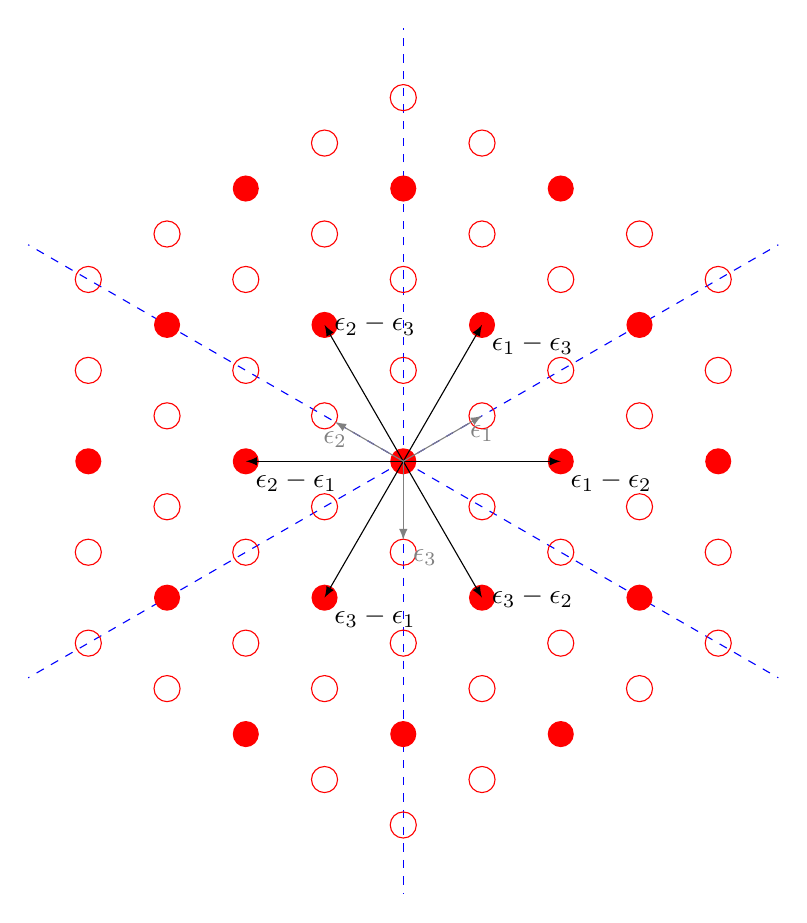
\begin{tikzpicture}[>=latex]
\pgfmathsetmacro\ax{2}
\pgfmathsetmacro\ay{0}
\pgfmathsetmacro\bx{2 * cos(120)}
\pgfmathsetmacro\by{2 * sin(120)}
\pgfmathsetmacro\lax{2*\ax/3 + \bx/3}
\pgfmathsetmacro\lay{2*\ay/3 + \by/3}
\pgfmathsetmacro\lbx{\ax/3 + 2*\bx/3}
\pgfmathsetmacro\lby{\ay/3 + 2*\by/3}

\foreach \k in {1,...,6} {
  \draw[blue,dashed] (0,0) -- +(\k * 60 + 30:5.5);
}
% \fill[blue!25] (0,0) -- (30:4 * \lby) -- (0,4 * \lby) -- cycle;
\begin{scope}
\clip (90:5) \foreach \k in {1,...,6} { -- ++([rotate=\k * 60 + 60]90:5) };
\foreach \na in {-3,...,2} {
  \foreach \nb in {-3,...,2} {
    \node[circle,fill=red] at (\na * \ax + \nb * \bx, \na * \ay + \nb * \by) {};
    \node[circle,draw=red] at (\lax + \na * \ax + \nb * \bx, \lay + \na * \ay + \nb * \by) {};
    \node[circle,draw=red] at (\lbx + \na * \ax + \nb * \bx, \lby + \na * \ay + \nb * \by) {};
  }
}
\end{scope}
\draw[black,->] (0,0) -- (\ax,\ay) node[below right]
{\(\epsilon_1-\epsilon_2\)};
\draw[black,->] (0,0) -- ({2*cos(60)}, {2*sin(60)}) node[below right] {\(\epsilon_1-\epsilon_3\)};
\draw[black,->] (0,0) -- (\bx,\by) node[right]
{\(\epsilon_2-\epsilon_3\)};
\draw[black,->] (0,0) -- ({-1*\ax},{-1*\ay}) node[below right]
{\(\epsilon_2-\epsilon_1\)};
\draw[black,->] (0,0) -- ({-2*cos(60)}, {-2*sin(60)}) node[below right] {\(\epsilon_3-\epsilon_1\)};
\draw[black,->] (0,0) -- ({-1*\bx},{-1*\by}) node[right]
{\(\epsilon_3-\epsilon_2\)};
\draw[gray,->] (0,0) -- ({\lax},{\lay}) node[below] {\(\epsilon_1\)};
\draw[gray,->] (0,0) -- ({cos(150)},{sin(150)}) node[below] {\(\epsilon_2\)};
\draw[gray,->] (0,0) -- (0,-1) node[below right] {\(\epsilon_3\)};
%\draw[->] (0,0) -- (\lbx,\lby) node[below right] {\(\lambda_2\)};
%\node at (0:5) {\(\rho_2\)};
%\node at (120:5) {\(\rho_1\)};
%\node at (180:5) {\(\rho_{12}\)};
%\node at (-120:5) {\(\rho_{121} = \rho_{212}\)};
%\node at (-60:5) {\(\rho_{21}\)};
\end{tikzpicture}
\caption{Weight lattice for \(\sl_3\). Choice of simple roots
  \(\alpha_1, \alpha_2\) are given by black arrows.}
  \end{figure}
\todo{Add
  images}
Thus, we can visualize a root string as a line through the
lattice. For instance, for \(\alpha \in \roots\), \[
  W := \bigoplus_{\substack{k \in \Z \\ \alpha+k(\epsilon_2-\epsilon_1)}} \g_{\alpha+k(\epsilon_2-\epsilon_1)}
\]
is symmetric about the line \(\{L \st \langle E_{1,1}-E_{2,2}, L
\rangle = 0\}\) and is thus preserved by reflection across said
line. 
\begin{prop}
  \cite{fulton}*{Prop 12.15} All eigenvalues of any irreducible
  finite-dimensional representation 
  of \(\sl_3(F)\) must lie in the weight lattice \(\weightlattice
  \subset \h^*\), that is, the lattice generated by the \(\epsilon_i\)
  and must be congruent 
  modulo the lattice \(\rootlattice \subset \h^*\) generated by the
  \(\epsilon_i-\epsilon_j\). 
\end{prop}
\begin{prop}
  \cite{fulton}*{Prop 12.18} Let \(V\) be any irreducible,
  finite-dimensional representation of \(\sl_3(F)\). Then, for some
  \(\alpha \in \weightlattice \subset \h^*\), the set of eigenvalues
  occurring in \(V\) is exactly the set of linear functionals
  congruent to \(\alpha\) modulo the lattice \(\rootlattice\) and
  lying in the hexagon with vertices the images of \(\alpha\) under
  the group generated by reflections in the lines \(\{L \st \langle
  E_{i,i}-E_{j,j},L \rangle = 0\}\). 
\end{prop}
\todo{Fill in proofs for these propositions.}
From this, we see that, given our choice of \(\ell\), it must be that
any heighest weight vector will lie in the region cut out by the
inequalities \(\langle
E_{1,1}-E_{2,2},L \rangle \geq 0\) and \(\langle E_{2,2}-E_{3,3},L
\rangle \geq 0\). In other words, it must be of the form \[
  (a+b)\epsilon_1 + b \epsilon_2 = a \epsilon_1 - b \epsilon_3
\]
Thus, we have reason to believe.
\begin{thm}\label{pair-gives-unique-irred-sl3-rep}
  For any pair of natural numbers \(a,b\), there exists a unique
  irreducible, finite-dimensional representation \(\Gamma_{a,b}\)of
  \(\sl_3(F)\) with highest weight \(a\epsilon_1-b\epsilon_3\).
\end{thm}
To prove this theorem, we will construct such representations
explicitly. Thus, let us look at some examples.
\begin{example}
  Consider the standard representation of \(\sl_3(\C)\) on \(V \isom
  \C^3\) with basis \(\{e_1,e_2,e_3\}\) with associated eigenvalues
  \(\epsilon_1, \epsilon_2, \)  and \(\epsilon_3\) since, for \[
    h = \left(
      \begin{array}{ccc}
        a_1&&\\
           &a_2&\\
        &&a_3
      \end{array}
\right) e_i = a_i e_i = \epsilon_i(h) e_i
  \]
  \begin{figure}[h]
    \centering
    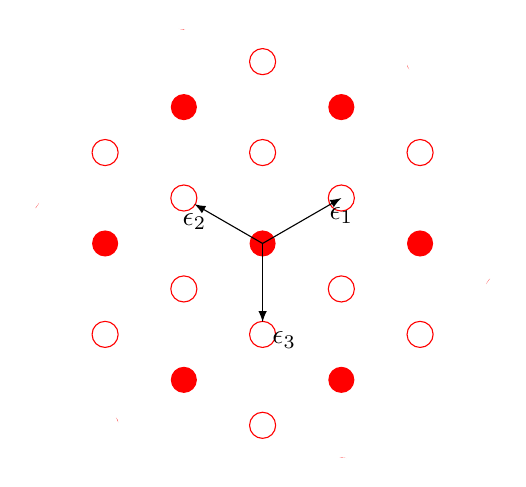
\begin{tikzpicture}[>=latex]
\pgfmathsetmacro\ax{2}
\pgfmathsetmacro\ay{0}
\pgfmathsetmacro\bx{2 * cos(120)}
\pgfmathsetmacro\by{2 * sin(120)}
\pgfmathsetmacro\lax{2*\ax/3 + \bx/3}
\pgfmathsetmacro\lay{2*\ay/3 + \by/3}
\pgfmathsetmacro\lbx{\ax/3 + 2*\bx/3}
\pgfmathsetmacro\lby{\ay/3 + 2*\by/3}

% \foreach \k in {1,...,6} {
%   \draw[blue,dashed] (0,0) -- +(\k * 60 + 30:5.5);
% }
% \fill[blue!25] (0,0) -- (30:4 * \lby) -- (0,4 * \lby) -- cycle;
\begin{scope}
\clip (54:3) \foreach \k in {1,...,6} { -- ++([rotate=\k * 60 + 60]54:3) };
\foreach \na in {-3,...,2} {
  \foreach \nb in {-3,...,2} {
    \node[circle,fill=red] at (\na * \ax + \nb * \bx, \na * \ay + \nb * \by) {};
    \node[circle,draw=red] at (\lax + \na * \ax + \nb * \bx, \lay + \na * \ay + \nb * \by) {};
    \node[circle,draw=red] at (\lbx + \na * \ax + \nb * \bx, \lby + \na * \ay + \nb * \by) {};
  }
}
\end{scope}
% \draw[black,->] (0,0) -- (\ax,\ay) node[below right]
% {\(\epsilon_1-\epsilon_2\)};
% \draw[black,->] (0,0) -- ({2*cos(60)}, {2*sin(60)}) node[below right] {\(\epsilon_1-\epsilon_3\)};
% \draw[black,->] (0,0) -- (\bx,\by) node[right]
% {\(\epsilon_2-\epsilon_3\)};
% \draw[black,->] (0,0) -- ({-1*\ax},{-1*\ay}) node[below right]
% {\(\epsilon_2-\epsilon_1\)};
% \draw[black,->] (0,0) -- ({-2*cos(60)}, {-2*sin(60)}) node[below right] {\(\epsilon_3-\epsilon_1\)};
% \draw[black,->] (0,0) -- ({-1*\bx},{-1*\by}) node[right]
% {\(\epsilon_3-\epsilon_2\)};
\draw[black,->] (0,0) -- ({\lax},{\lay}) node[below] {\(\epsilon_1\)};
\draw[black,->] (0,0) -- ({cos(150)},{sin(150)}) node[below] {\(\epsilon_2\)};
\draw[black,->] (0,0) -- (0,-1) node[below right] {\(\epsilon_3\)};
%\draw[->] (0,0) -- (\lbx,\lby) node[below right] {\(\lambda_2\)};
%\node at (0:5) {\(\rho_2\)};
%\node at (120:5) {\(\rho_1\)};
%\node at (180:5) {\(\rho_{12}\)};
%\node at (-120:5) {\(\rho_{121} = \rho_{212}\)};
%\node at (-60:5) {\(\rho_{21}\)};
\end{tikzpicture}
    \caption{Weight diagram for \(V\), the standard representation of
      \(\sl_3(\C)\)}
  \end{figure}
  Consider also its
  dual, \(V^*\), with dual basis \(\{e_1^*, e_2^*, e_3^*\}\) and
  associated eigenvalues \(-\epsilon_1, -\epsilon_2,\) and
  \(-\epsilon_3\).
  \begin{figure}[h]
    \centering
    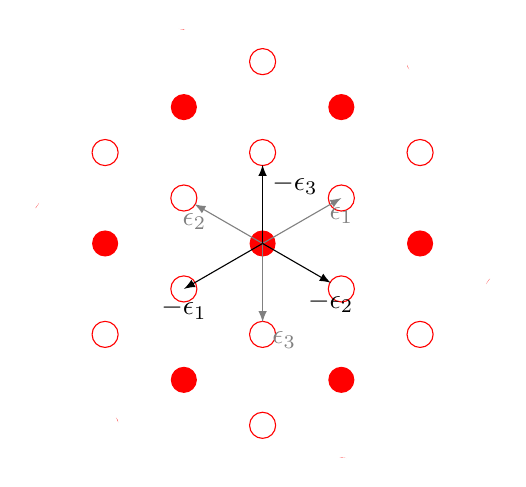
\begin{tikzpicture}[>=latex]
\pgfmathsetmacro\ax{2}
\pgfmathsetmacro\ay{0}
\pgfmathsetmacro\bx{2 * cos(120)}
\pgfmathsetmacro\by{2 * sin(120)}
\pgfmathsetmacro\lax{2*\ax/3 + \bx/3}
\pgfmathsetmacro\lay{2*\ay/3 + \by/3}
\pgfmathsetmacro\lbx{\ax/3 + 2*\bx/3}
\pgfmathsetmacro\lby{\ay/3 + 2*\by/3}

% \foreach \k in {1,...,6} {
%   \draw[blue,dashed] (0,0) -- +(\k * 60 + 30:5.5);
% }
% \fill[blue!25] (0,0) -- (30:4 * \lby) -- (0,4 * \lby) -- cycle;
\begin{scope}
\clip (54:3) \foreach \k in {1,...,6} { -- ++([rotate=\k * 60 + 60]54:3) };
\foreach \na in {-3,...,2} {
  \foreach \nb in {-3,...,2} {
    \node[circle,fill=red] at (\na * \ax + \nb * \bx, \na * \ay + \nb * \by) {};
    \node[circle,draw=red] at (\lax + \na * \ax + \nb * \bx, \lay + \na * \ay + \nb * \by) {};
    \node[circle,draw=red] at (\lbx + \na * \ax + \nb * \bx, \lby + \na * \ay + \nb * \by) {};
  }
}
\end{scope}
% \draw[black,->] (0,0) -- (\ax,\ay) node[below right]
% {\(\epsilon_1-\epsilon_2\)};
% \draw[black,->] (0,0) -- ({2*cos(60)}, {2*sin(60)}) node[below right] {\(\epsilon_1-\epsilon_3\)};
% \draw[black,->] (0,0) -- (\bx,\by) node[right]
% {\(\epsilon_2-\epsilon_3\)};
% \draw[black,->] (0,0) -- ({-1*\ax},{-1*\ay}) node[below right]
% {\(\epsilon_2-\epsilon_1\)};
% \draw[black,->] (0,0) -- ({-2*cos(60)}, {-2*sin(60)}) node[below right] {\(\epsilon_3-\epsilon_1\)};
% \draw[black,->] (0,0) -- ({-1*\bx},{-1*\by}) node[right]
% {\(\epsilon_3-\epsilon_2\)};
\draw[gray,->] (0,0) -- ({\lax},{\lay}) node[below] {\(\epsilon_1\)};
\draw[gray,->] (0,0) -- ({cos(150)},{sin(150)}) node[below] {\(\epsilon_2\)};
\draw[gray,->] (0,0) -- (0,-1) node[below right] {\(\epsilon_3\)};
\draw[black,->] (0,0) -- ({-1*\lax},{-1*\lay}) node[below] {\(-\epsilon_1\)};
\draw[black,->] (0,0) -- ({-1*cos(150)},{-1*sin(150)}) node[below] {\(-\epsilon_2\)};
\draw[black,->] (0,0) -- (0,1) node[below right] {\(-\epsilon_3\)};

% \draw[->] (0,0) -- (\lbx,\lby) node[below right] {\(\lambda_2\)};
%\node at (0:5) {\(\rho_2\)};
%\node at (120:5) {\(\rho_1\)};
%\node at (180:5) {\(\rho_{12}\)};
%\node at (-120:5) {\(\rho_{121} = \rho_{212}\)};
%\node at (-60:5) {\(\rho_{21}\)};
\end{tikzpicture}
    
    \caption{Weight diagram for \(V^*\), the dual representation of
      the standard representation of \(\sl_3(\C)\)}
  \end{figure}

Using weight diagrams \todo{Actually insert these},
  one can see that \(\operatorname{Sym}^2 V\) and
  \(\operatorname{Sym}^2 V^*\), whose weights are the pairwise sums of
  the weights of \(V\) and \(V^*\), respectively, are both
  irreducible.
  \begin{figure}[h]
    \centering
    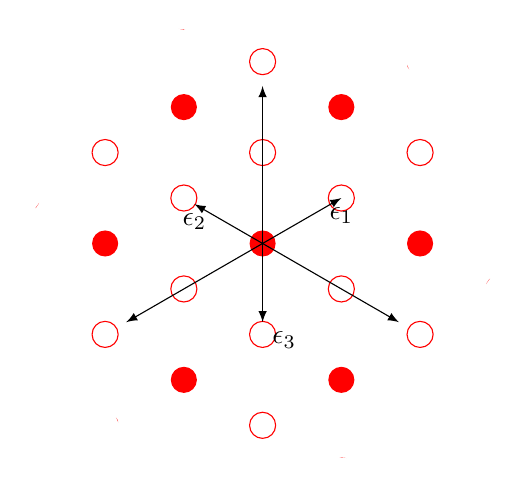
\begin{tikzpicture}[>=latex]
\pgfmathsetmacro\ax{2}
\pgfmathsetmacro\ay{0}
\pgfmathsetmacro\bx{2 * cos(120)}
\pgfmathsetmacro\by{2 * sin(120)}
\pgfmathsetmacro\lax{2*\ax/3 + \bx/3}
\pgfmathsetmacro\lay{2*\ay/3 + \by/3}
\pgfmathsetmacro\lbx{\ax/3 + 2*\bx/3}
\pgfmathsetmacro\lby{\ay/3 + 2*\by/3}

% \foreach \k in {1,...,6} {
%   \draw[blue,dashed] (0,0) -- +(\k * 60 + 30:5.5);
% }
% \fill[blue!25] (0,0) -- (30:4 * \lby) -- (0,4 * \lby) -- cycle;
\begin{scope}
\clip (54:3) \foreach \k in {1,...,6} { -- ++([rotate=\k * 60 + 60]54:3) };
\foreach \na in {-3,...,2} {
  \foreach \nb in {-3,...,2} {
    \node[circle,fill=red] at (\na * \ax + \nb * \bx, \na * \ay + \nb * \by) {};
    \node[circle,draw=red] at (\lax + \na * \ax + \nb * \bx, \lay + \na * \ay + \nb * \by) {};
    \node[circle,draw=red] at (\lbx + \na * \ax + \nb * \bx, \lby + \na * \ay + \nb * \by) {};
  }
}
\end{scope}
% \draw[black,->] (0,0) -- (\ax,\ay) node[below right]
% {\(\epsilon_1-\epsilon_2\)};
% \draw[black,->] (0,0) -- ({2*cos(60)}, {2*sin(60)}) node[below right] {\(\epsilon_1-\epsilon_3\)};
% \draw[black,->] (0,0) -- (\bx,\by) node[right]
% {\(\epsilon_2-\epsilon_3\)};
% \draw[black,->] (0,0) -- ({-1*\ax},{-1*\ay}) node[below right]
% {\(\epsilon_2-\epsilon_1\)};
% \draw[black,->] (0,0) -- ({-2*cos(60)}, {-2*sin(60)}) node[below right] {\(\epsilon_3-\epsilon_1\)};
% \draw[black,->] (0,0) -- ({-1*\bx},{-1*\by}) node[right]
% {\(\epsilon_3-\epsilon_2\)};
\draw[black,->] (0,0) -- ({\lax},{\lay}) node[below] {\(\epsilon_1\)};
\draw[black,->] (0,0) -- ({cos(150)},{sin(150)}) node[below] {\(\epsilon_2\)};
\draw[black,->] (0,0) -- (0,-1) node[below right] {\(\epsilon_3\)};
\draw[black,->] (0,0) -- (0,2);
\draw[black,->] (0,0) -- ({2*cos(210)},{2*sin(210)});
\draw[black,->] (0,0) -- ({2*cos(330)},{2*sin(330)});
%\draw[->] (0,0) -- (\lbx,\lby) node[below right] {\(\lambda_2\)};
%\node at (0:5) {\(\rho_2\)};
%\node at (120:5) {\(\rho_1\)};
%\node at (180:5) {\(\rho_{12}\)};
%\node at (-120:5) {\(\rho_{121} = \rho_{212}\)};
%\node at (-60:5) {\(\rho_{21}\)};
\end{tikzpicture}
    \caption{Weight diagram for \(\operatorname{Sym}^2 V^*\)}
  \end{figure}
  A more interesting analysis comes from examining \(V
  \otimes V^*\).

  One can quickly check that the weights of \(V \otimes V^*\) are
  \(\{\epsilon_1 \pm \epsilon_2, \epsilon_1 \pm \epsilon_3, \epsilon_2
  \pm \epsilon_3\}\), each with multiplicity \(1\), and \(0\) with
  multiplicity \(3\). Since the linear map \[
    v \otimes u^* \mapsto \langle v, u^* \rangle = u^*(v)
  \]
  has a non-trivial kernel. One can easily check that this map is
  equivalent to the trace since \(V \otimes V^* \isom \Hom(V,V) \isom
  M_3(\C)\) and thus the kernel is all traceless matrices, ie
  the adjoint representation of \(\sl_3(\C)\), which is an irreducible
  \(\sl_3(\C)\)-representation. Thus, \[
    V \otimes V^* \isom \sl_3(\C) \oplus \C
  \]
\end{example}
We will also need the following lemma
\begin{lem}
  Given representations \(V\) and \(W\) with highest weight vectors
  \(v,w\) with weights \(\alpha,\beta\), respectively, then \(v
  \otimes w \in V \otimes W\) is a highest weight vector of weight
  \(\alpha + \beta\).
\end{lem}
\begin{proof}
  Consider that, for \(E_{i,j}\) with \(i \leq j\), we get \[
    E_{i,j}.(v \otimes w) = E_{i,j}.v \otimes w + v \otimes E_{i,j}.w
    = 0 + 0 = 0
  \]
  and, for \(H \in \h\), we get
  \begin{align*}
    H.(v \otimes w) & = H.v \otimes w + v \otimes H.w \\
                    & = \alpha(H)v \otimes w + v \otimes \beta(H) w \\
    & = (\alpha(H)+\beta(H)) (v \otimes w)
  \end{align*}
\end{proof}
Thus, from the example and the lemma, we get
\begin{prop}
  Given standard representation \(V\), we have the following
  \begin{enumerate}
  \item \(V\) has a highest weight vector with weight
    \(\epsilon_1\).
  \item \(V^*\) has a highest weight vector with weight
    \(-\epsilon_3\).
  \item \(\operatorname{Sym}^n V\) has a highest weight vector with
    weight \(n \cdot \epsilon_1\).
  \item \(\operatorname{Sym}^n V^*\) has a highest weight vector with
    weight \(-n\cdot \epsilon_3\).
  \end{enumerate}
\end{prop}
\begin{proof}[Proof of Theorem \ref{pair-gives-unique-irred-sl3-rep}]
  Let \(V\) be the standard representation of \(\sl_3(F)\). Then,
  \(\operatorname{Sym}^a V \otimes \operatorname{Sym}^b V^*\) contains
  an irreducible subrepresentation generated by the highest weight
  vector with weight \(a \epsilon_1 - b \epsilon_3\).

  To show uniqueness, let \(V,W\) be two \(\sl_3(F)\)-representations
  with highest weight \(\alpha\) and corresponding highest weight
  vectors \(v,w\). Then. consider \((v,w) \in V \oplus W\) will be a
  highest weight vector with highest weight \(\alpha\). Let \(U\) be
  the irreducible subrepresentation generated by \((v,w)\). Then, we
  have non-zero projections between irreducibles, \[
    \pi_1 \from U \to V, \ \ \pi_2 \from U \to W
  \]
  which, by Schur's lemma, must be isomorphisms. Thus, \(V \isom U
  \isom W\).
\end{proof}
In fact, we can more explicitly construct the representations
\(\Gamma_{a,b}\), most easily using the Weyl Character Formula, which
has not been proven yet. However, the final result will be given by
first considering the contraction map
\begin{align*}
    \iota_{a,b} \from \operatorname{Sym}^a V \otimes
  \operatorname{Sym}^b V^*
  & \to \operatorname{Sym}^{a-1} V \otimes \operatorname{Sym}^{b-1} V^* \\
  (v_1 \cdots v_a) \otimes (v_1^* \cdots v_b^*)
  & \mapsto \sum \langle v_i, v_j^* \rangle(v_1 \cdots \hat{v_i}
    \cdots v_a) \otimes (v_1^* \cdots \hat{v_j^*} \cdots v_b^*)
\end{align*}
Such a map is surjective and the codomain cannot have eigenvalue \(a
\epsilon_1 - b \epsilon_3\), so \(\Gamma_{a,b} \subset \ker
\iota_{a,b}\). In fact, using the Weyl Character Formula, we
immediately conclude
\begin{prop}
  \(\ker \iota_{a,b} = \Gamma_{a,b}\).
\end{prop}
Also, as an immediate corollary, we conclude
\begin{cor}
  If \(b \leq a\), \(\operatorname{Sym}^a V \otimes
  \operatorname{Sym}^b V^* \isom \bigoplus_{i=0}^b \Gamma_{a-i,b-i}\)
  and similarly if \(a \leq b\).
\end{cor}
\section{More Structure Theory of Semisimple Lie Algebras}
We state some results here without proof since they can be superseced
by Serre's theorem. However, we wish to establish that maximal toral
subalgebras and Cartan subalgebras coincide for semisimple Lie
algebras. Along the way, we establish a few other distinguished
subalgebras of semisimple Lie algebras which appear throughout the
literature on Lie algebras.
\begin{prop}
  \cite{humph}*{p 74} Let \(\g\) be a semisimple Lie algebra, \(\h \subset \g\) a maximal
  toral subalgebra, and \(\roots\) the root system of \(\g\) relative
  to \(\h\). Fix a base \(\simpleroots\) of \(\roots\). Then, \(\g\)
  is generated as a Lie algebra by the root spaces \(\g_\alpha,
  \g_{-\alpha}\) for \(\alpha \in \simpleroots\). Equivalently, \(\g\)
  is generated by arbitrary nonzero root vectors \(x_\alpha \in
  \g_\alpha, y_\alpha \in \g_{-\alpha}\) for \(\alpha \in \simpleroots\).
\end{prop}
\begin{thm}
  \cite{humph}*{p 75} Let \(\g,\g'\) be simple Lie algebra over a field \(F\) with
  respective maximal toral subalgebras \(\h,\h'\) and corresponding
  root systems \(\roots,\roots'\). Suppose there is an isomorphism of
  \(\roots\) onto \(\roots'\) given by \(\alpha \mapsto \alpha'\)
  inducing \(\pi \from \h \to \h'\). Fix a 
  base \(\simpleroots \subset \roots\) so that \(\roots' = \{\alpha'
  \st \alpha \in \simpleroots\}\) is a base of \(\roots'\). For each
  \(\alpha \in \simpleroots, \alpha' \in \simpleroots'\), choose
  arbitrary (nonzero) \(x_\alpha \in \g_\alpha, x_\alpha' \in
  \g_\alpha'\), that is, choose an arbitrary Lie algebra isomoprhism
  \(\pi_\alpha \from \g_\alpha \to \g_\alpha'\). Then, there eixsts a
  unique isomorphism \(\pi \from \g \to \g'\) extending \(\pi \from \h
  \to \h'\) and extending all of the \(\pi_\alpha\), \(\alpha \in
  \simpleroots\).  \[
    \begin{tikzcd}
      \h \ar[d,"\pi"] \ar[r]& \g \ar[d,dashed, "\pi"]& \ar[l] \ar[d,"\pi_\alpha"] \g_\alpha \\
      \h' \ar[r] & \g' & \ar[l] \g_\alpha'
    \end{tikzcd}
  \]
\end{thm}
\begin{prop}
  \cite{humph}*{p 77} Given \(\g\) as above, but not necessarily simple, fix \(0 \neq
  x_\alpha \in \g_\alpha\) for \(\alpha \in \simpleroots\) and let
  \(y_\alpha \in \g_{-\alpha}\) satisfy \([x_\alpha, y_\alpha] =
  h_\alpha\). Then, there exists an automorphism \(\sigma\) of \(\g\)
  of order \(2\), satisfying, for \(\alpha \in \simpleroots, h \in
  \h\), \(\sigma(x_\alpha) = -y_\alpha,
  \sigma(y_\alpha) = -x_\alpha, \sigma(h) = -h\).
\end{prop}
\begin{proof}
  This follows from the fact that any automorphism of \(\roots\) can
  be extended to \(\Aut \roots\), so in particular, the map sending
  each root to its negative is in \(\Aut \roots\).
\end{proof}
\begin{defn}
  Let \(t \in \End V\), \(a\) be a root of the characteristic
  polynomial of \(t\) with multiplicity \(m\), and \(V_a := \ker (t-a
  \cdot 1)^m\). Then, given an \(x \in \g\), a Lie algebra over
  algebraically closed field \(F\) , we call \(\g_0(\ad x)\) for \(\ad x
  \in \End \g\) an \de{Engel subalgebra}.
\end{defn}
\begin{lem}
  \cite{humph}*{p 78} If \(a,b \in F\), then \([\g_a(\ad x), \g_b(\ad x)] \subset
  \g_{a+b}(\ad x)\). In particular, \(\g_0(\ad x)\) is a subalgebra of
  \(\g\), and when \(\Char F = 0, a \neq 0\), each element of
  \(\g_a(\ad x)\) is \(\ad\)-nilpotent. Thus, an Engel subalgebra is
  actually an algebra.
\end{lem}
\begin{proof}
  Compute the expansion \[
    (\ad x-a-b)^m[y,z] = \sum_{i=0}^m \binom{m}{i}[(\ad x - a)^i(y),
    (\ad x - b)^{m-i}(z)]
  \] for \(y \in \g_a(\ad x), z \in
  \g_b(\ad x)\). For sufficiently large \(m\) the expression will be \(0\).
\end{proof}
\begin{lem}
  \cite{humph}*{p 79} Let \(\g'\) be a subalgebra of \(\g\). Choose \(z \in \g'\) such
  that \(\g_0(\ad z)\) is minimal in the collection of all \(\g_0(\ad
  x)\) for \(x \in \g'\). Suppose that \(\g' \subset \g_0(\ad
  z)\). Then, \(\g_0(\ad z) \subset \g_0(\ad x)\) for all \(x \in \g'\).
\end{lem}
\begin{lem}
  \cite{humph}*{p 79} If \(\g'\) is a subalgebra of \(\g\) containing an Engel subalgebra,
  then \(N_\g(\g') = \g'\). In particular, Engel subalgebras are
  self-normalizing.
\end{lem}
\begin{defn}
  A \de{Cartan subalgebra} (CSA) of a Lie algebra \(\g\) is a nilpotent
  subalgebra which equals its normalizer in \(\g\). 
\end{defn}
\begin{thm}
  \cite{humph}*{p 80} Let \(\h\) be a subalgebra of Lie algebra \(\g\). Then, \(\h\) is a
  CSA of \(\g\) if and only if \(\h\) is a minimal Engel subalgebra.
\end{thm}
\begin{cor}
  \cite{humph}*{p 80} Let \(\g\) be semisimple over \(F\) with \(\Char F = 0\). Then, the
  CSA's of \(\g\) are precisely the maximal toral subalgebras of \(\g\).
\end{cor}
\begin{prop}
  \cite{humph}*{p 81} Let \(\phi \from \h \to \h'\) be a surjective Lie algebra
  homomorphism.
  \begin{enumerate}
  \item If \(\h\) is a CSA of \(\g\), then \(\phi(\h)\) is a CSA of
    \(\g'\).
  \item If \(\h'\) is a CSA of \(\g'\) and \(K = \phi^{-1}(\h')\),
    then any CSA \(\h\) of \(K\) is also a CSA of \(\g\).
  \end{enumerate}
\end{prop}
\begin{defn}
  A \de{Borel subalgebra} of a Lie algebra \(\g\) is a maximal
  solvable subalgebra of \(\g\).
\end{defn}
\begin{defn}
  Let \(\g\) be a finite dimensional semisimple Lie algebra over
  \(\C\) and let \(\h\) be a CSA of \(\g\). Then, \(\g\) has
  \de{triangular decomposition} \[
    \g = \n^{-} \oplus \h \oplus \n
  \]
  where \(\n^{-} = \bigoplus_{\alpha \in \roots^-} \g_\alpha\) and
  \(\n = \bigoplus_{\alpha \in \roots^+} \g_\alpha\). 
\end{defn}
\begin{prop}
  The \(\n^-\) and \(\n\) in the triangular decomposition are
  subalgebras of \(\g\).
\end{prop}
\begin{proof}
  The sum of two positive roots is still positive. So, for
  \(\alpha,\beta \in \roots^+\), we have \[
    [\g_\alpha, \g_\beta] \subset \g_{\alpha+\beta} \subset \n
  \]
  and so \(\n\) is a subalgebra. Similarly for \(\n^-\).
\end{proof}
\begin{prop}
  \begin{enumerate}
  \item   \(\b = \h \oplus \n\) is a Borel subalgebra, called \de{standard}
    relative to \(\h\).
  \item \(\n\) is an ideal of \(\b\).
  \item \(\b/\n \isom \h\).
  \end{enumerate}
\end{prop}
\begin{proof}
  For (a), we first observe that \[
    [\b,\b] = [\h+\n, \h+\n] \subset \h+\n = \b
  \]
  because \(\h,\n\) are subalgebras and \([\h,\n] \subset \n\). Thus,
  \(\b\) is a subalgebra.\\

  Let \(\g'\) be any subalgebra of \(\g\) properly containing
  \(\b\). Since it is a subalgebra containing \(\h\), \(\g'\) must be
  stable under the \(\ad \h\) action, and so it must include some
  \(\g_\alpha\) with \(\alpha \prec 0\). However, then \(\g'\)
  contains a copy of \(\sl_2\) generated by \(\{x_\alpha, y_\alpha,
  [x_\alpha,y_\alpha]\}\) for \(x_\alpha \in \g_{-\alpha}, y_\alpha
  \in \g_\alpha\). Since \(\sl_2\) is simple, \(\g'\) cannot be
  solvable. \\

  For (b), we observe \[
    [\n,\b] = [\n,\n+\h] \subset \n
  \]

  For (c), we compute \[
    \b/\n = (\h+\n)/\n \isom \h/(\h \intersect \n) \isom \h
  \]
  because \(\h \intersect \n = 0\). 
\end{proof}
\begin{prop}
  \cite{humph}*{pp 83--84}
  \begin{enumerate}
  \item If \(\b\) is a Borel subalgebra of \(\g\), then \(\b =
    N_\g(\b)\).
  \item If \(\rad \g \neq \g\), then the Borel subalgebras of \(\g\)
    are in natural one-to-one correspondence with those of the
    semisimple Lie algebra \(\g / \rad \g\).
  \item Let \(\g\) be semisimple with CSA \(\h\) and root system
    \(\roots\). All standard Borel subalgebras of \(\g\) relative to
    \(\h\) are conugate under inner automorphisms of \(\Aut \g\).
  \end{enumerate}
\end{prop}
\begin{thm}
  \cite{humph}*{p 84} The Borel subalgebras of an arbitrary Lie algebra \(\g\) are all
  conjugate under inner automorphisms of \(\Aut \g\).
\end{thm}
\begin{cor}
  \cite{humph}*{p 84} The Cartan subalgebras of an arbitrary Lie algebra \(\g\) are
  conjugate under inner automorphisms of \(\Aut \g\).
\end{cor}
\section{Universal Enveloping Algebra}
In this section, we will construct an associative algebra \(\U(\g)\)
such that the representation theory of \(\U(\g)\) is the same as the
representation theory of \(\g\).
\begin{defn}
  Let \(V\) be a finite dimensional vector space over a field
  \(F\). Then, we define
  \begin{align*}
    \T^0 V & = F \\
    \T^1 V & = V \\
    \T^2 V & = V \otimes V \\
    \vdots & \\
    \T^n V & = \underbrace {V \otimes \cdots \otimes V }_{n \text{ times}}
  \end{align*}
  and say \(\T(V) = \Dunion \T^k V\) equipped with the product
  \begin{align*}
    \T^m V \times \T^n V & \to T^{m+n}V\\
    (v_1 \otimes \cdots \otimes v_m) \cdot (w_1 \otimes \cdots \otimes
    w_n) & \mapsto v_1 \otimes \cdots \otimes v_m \otimes w_1 \otimes
           \cdots \otimes w_n
  \end{align*}
  is called the \de{tensor algebra} on \(V\).
\end{defn}
\begin{prop}
  Let \(V\) be a finite dimensional vector space and \(A\) an
  associative unital algebra over \(F\). Then, we have the
  following universal property:
  \[
    \begin{tikzcd}
      V \ar[r,"\iota"] \ar[rd, "\phi"]& \T(V) \ar[d, dashed, "\exists
      \unique \Phi"] \\ 
      & A
    \end{tikzcd}
  \]
  In words, for any \(F\)-linear map \(\phi \from V \to A\) and
  \(\iota \from V \to \T(V)\) sending \(v \mapsto v \in T^1 V\), there
  is a unique homomorphism of \(F\)-algebra \(\Phi \from \T(V) \to A\)
  such that \(\Phi \circ \iota = \phi\).
\end{prop}
\begin{defn}
  Let \(\g\) be a Lie algebra. Then, consider the ideal \(J = \langle
  x \otimes y - y \otimes x - [x,y] \st x,y \in \g \rangle\) in
  \(\T(\g)\). We define \[
    \U(\g) = T(\g) / J
  \]
  and call such a quotient the \de{universal enveloping algebra} of \(\g\).
\end{defn}
\begin{example}
  Let \(\g\) be an \(n\)-dimensional abelian Lie algebra over \(\C\)
  with basis \(\{x_1, \ldots, x_n\}\) and \([x_i,x_j] = 0\). Then, \(J
  \ideal \T(\g)\) is given by \(J = \langle x \otimes y - y \otimes x
  \st x,y \in \g
  \rangle\). Therefore, \(\U(\g)\) is commutative and generated by
  \(1, x_1 ,\ldots, x_n\). Thus, \(\U(\g) \isom \C[x_1, \ldots,
  x_n]\). 
\end{example}
\begin{prop}
  Let \(\g\) be an arbitrary Lie algebra. Then, if \(\iota \from \g
  \to \U(\g)\) is a linear map satisyfing \[
    \iota([x,y]) = \iota(x)\iota(y) - \iota(y)\iota(x), \ x,y \in \g
  \]
  and \(\phi \from \g \to A\) satisfies the same property for \(A\) an
  associative unital \(F\)-algebra, then we have the following
  universal property
  \[
    \begin{tikzcd}
      \g \ar[rd, "\phi"] \ar[r, "\iota"] & \U(\g) \ar[d, dashed,
      "\exists \unique \Phi"]\\
      & A
    \end{tikzcd}
  \]
  that is, there is a unique \(F\)-algebra homomorphism \(\Phi \from
  \U(\g) \to A\) such that \(\Phi \circ \iota = \phi\).
\end{prop}
\begin{rmk}
  Note that we have not shown that \(\iota\) is injective, but we will
  do so later with the PBW Theorem.
\end{rmk}
\begin{prop}
  There is a bijective correspondence between representations \(\theta
  \from \g \to[] \gl(V)\) and representations \(\phi \from \U(\g)
  \to \End V\). Corresponding representations are
  related by the condition \[
    \phi(\iota(x)) = \theta(x) \text{ for all }x \in \g
  \]
  where \(\iota \from \g \to \U(\g)\) is the standard inclusion.
\end{prop}
\begin{proof}
  Given \(\theta\) a representation of \(\g\), we have \[
    \begin{tikzcd}
      \g \ar[rd, "\theta"]\ar[r, "\iota"] & \U(\g) \ar[d, dashed,
      "\exists \unique \phi"] \\ 
      & \gl(V) = \End V
    \end{tikzcd}
  \]
  where \(\phi \from \U(\g) \to \End V\) is a representation of
  \(\U(\g)\). \\

  Conversely, given \(\phi\) a representation of \(\U(\g)\), we know
  that the linear map \(\iota \from \g \to \U(\g)\) has \[
    \iota(x)\iota(y)-\iota(y)\iota(x) = \iota([x,y]) \implies
    [\iota(x),\iota(y)] = \iota([x,y])
  \]
  if we define \([\cdot,\cdot] \from \U(\g)\times \U(\g) \to \U(\g)\)
  by \([x,y] = xy-yx\). Thus, \(\iota \from \g \to[] [\U(\g)]\), that
  is, \(\U(\g)\) with the extra Lie algebra structure, is a Lie
  algebra homomorphism. \[
    \begin{tikzcd}
      \g \ar[r, "\iota"] & \U(\g) \ar[d, "\phi"] \\
      & \End V
    \end{tikzcd} \implies
    \begin{tikzcd}
      \g \ar[r, "\iota"] \ar[rd, dashed, swap, "\phi \circ \iota"] &
      {[}\U(\g){]} \ar[d, "\phi"] \\ 
      & \gl(V)
    \end{tikzcd}
  \]
  Then, \(\phi \circ \iota\) is a representation 
\end{proof}
\begin{rmk}
  Note, the representations under consideration need not be
  finite-dimensional. In fact, it will turn out that a certain
  important class of representations called ``Verma modules'' will
  always be infinite-dimensional.
\end{rmk}
This construction will lead us to the all-important PBW Theorem, which
tells us how to obtain a basis for the universal enveloping algebra of
a Lie algebra.
\begin{thm}[Poincar\'{e}-Birkhoff-Witt Theorem]
  \cite{carter}*{Theorem 9.4} Let \(\g\) be a Lie algebra with basis
  \(\{x_i \st i \in I\}\). Let \(<\) be a total order on the index set
  \(I\). Let \(\iota \from \g \to \U(\g)\) be the natural linear map
  from \(\g\) to its enveloping algebra. We define \(y_i :=
  \iota(x_i)\). Then, the elements \[
    y_{i_1}^{r_1} \cdots y_{i_n}^{r_n}
  \]
  for all \(n \geq 0\), all \(r_i \geq 0\), and all \(i_1, \ldots, i_n
  \in I\) with \(i_1 < I_2 < \cdots < i_n\) form a basis for \(\U(\g)\).
\end{thm}
For the proof of this theorem, see \cite{carter}*{pp 155--159} or
\cite{humph}*{pp 93--94} (Note, \cite{humph} gives an equivalent
statement of the PBW Theorem and states this version as Corollary
C). The PBW Theorem has many important corollaries such as
\begin{cor}
  The map \(\iota \from \g \to \U(\g)\) is injective.
\end{cor}
\begin{proof}
  By the PBW Theorem, the elements \(y_i\) for \(i \in I\) are
  linearly independent. Since the \(x_i \in \g\) form a basis for
  \(\g\) and \(\iota(x_i) = y_i\), it must be that \(\ker \iota =
  \{0\}\).   
\end{proof}
\begin{cor}
  The subspace \(\iota(\g) \subset [\U(\g)]\) is isomorphic to
  \(\g\) as a Lie subalgebra.
\end{cor}
\begin{proof}
  From the corollary above, \(\iota \from \g \to \iota(\g)\) is
  bijective and \(y_i, i \in I\) form a basis of
  \(\iota(\g)\). Furthermore, \[
    [y_i,y_j] = [\iota(x_i), \iota(x_j)] = \iota([x_i,x_j]) \in \iota(\g)
  \]
  Thus, \(\iota(\g)\) is a Lie subalgebra of \([\U(\g)]\).
\end{proof}
\begin{cor}
  \(\U(\g)\) has no zero-divisors.
\end{cor}
\begin{proof}
  Take \(0 \neq a,b \in \U(\g)\). Then,
  \begin{align*}
    a & = \sum \lambda_{i_1, \ldots, i_n, r_1, \ldots, r_n}
        y_{i_1}^{r_1} \cdots y_{i_n}^{r_n}  \\
      & = \sum_{\substack{r_1 + \cdots + r_n = r \\ \text{ maximal degree}}} \lambda_{i_1, \ldots, i_n, r_1, \ldots, r_n}
        y_{i_1}^{r_1} \cdots y_{i_n}^{r_n} + \sum_{r_1 + \cdots + r_n
        < r} \lambda_{i_1, \ldots, i_n, r_1, \ldots, r_n}
    y_{i_1}^{r_1} \cdots y_{i_n}^{r_n} \\
      & = f(y_i) + \text{ sum of terms of smaller degree}\\
    b & = \sum \mu_{i_1, \ldots, i_n, r_1, \ldots, r_n}
        y_{i_1}^{r_1} \cdots y_{i_n}^{r_n}  \\
      & = \sum_{\substack{r_1 + \cdots + r_n = r \\ \text{ maximal degree}}} \mu_{i_1, \ldots, i_n, r_1, \ldots, r_n}
        y_{i_1}^{r_1} \cdots y_{i_n}^{r_n} + \sum_{r_1 + \cdots + r_n
        < r} \mu_{i_1, \ldots, i_n, r_1, \ldots, r_n}
    y_{i_1}^{r_1} \cdots y_{i_n}^{r_n} \\
      & = g(y_i) + \text{ sum of terms of smaller degree}
  \end{align*}
  Recall also, since \(\iota(\g)\) is a Lie subalgebra, \[
    y_i y_j - y_j y_i = [y_i,y_j] = \sum_k \nu_k y_k
  \]
  and so \todo{why?} \[
    f(y_i) g(y_i) = (fg)(y_i) + \text{a sum of terms of smaller degree.}
  \]
  Therefore, \[
    ab = (fg)(y_i) + \text{a sum of terms of smaller degree.}
  \]
  and since \(f \neq 0 \neq g\), we get \(fg \neq 0\). Thus, the PBW
  Theorem tells us that \(ab \neq 0\).
\end{proof}
\section{Irreducible Modules of Semisimple Lie Algebras}
\begin{lem}
  \cite{carter}*{Lemma 10.1} Let \(\g\) be a finite dimensional Lie algebra over \(\C\), and let
  \(\g'\) be a subalgebra of \(\g\). Then, there exists a unique
  algebra homomorphism \(\theta \from \U(\g') \to \U(\g)\) such that the
  following diagram commutes \[
    \begin{tikzcd}
      \g' \ar[d, "i"] \ar[r, "\iota_{\g'}"] & \U(\g') \ar[d, "\theta"] \\
      \g \ar[r,"\iota_{\g}"] & \U(\g)
    \end{tikzcd}
  \]
  where \(i\) is the embedding of \(\g'\) into \(\g\) and
  \(\iota_{\g'}, \iota_\g\) are the standard embeddings of a Lie
  algebra into its universal enveloping algebra. Furthermore, \(\theta\)
  is injective.
\end{lem}
\begin{proof}
  For \(x \in \g'\), the definition \[
    \theta(\iota_{\g'}(x)) = \iota_\g(i(x))
  \]
  is well-defined and, since \(\U(\g')\) is generated by
  \(\iota(\g')(\g')\), such a \(\theta\) is uniquely determined. To
  see existence, define one notices \[
    \begin{tikzcd}
      \g' \ar[r] \ar[d, "i"]& T(\g') \ar[d, dashed, "i^*"] \ar[r] & T(\g')/J'
      \isom \U(\g') \ar[d, dotted] \\
      \g \ar[r] & T(\g) \ar[r] & T(\g)/J \isom \U(\g)
    \end{tikzcd}
  \]
  since \(i^*(J') \subset J\), where \(J,J'\) are the ideals used to
  define the universal enveloping algebra. \\

  To see \(\theta\) is injective, let \(x_1, \ldots, x_r\) be a basis
  for \(\g'\) and \(0 \neq u \in \U(\g')\). Then, \(u\) is a non-zero
  linear combination of monomials 
  \(x_1^{e_1} \cdots x_r^{e_r}\). Then, let \(x_1, \ldots, x_r\) be
  part of a basis of \(\g\). The PBW theorem tells us that such a
  linear combination of monomials cannot be zero in \(\U(\g)\). Thus,
  \(\theta(u) \neq 0\) and so \(\ker \theta = 0\). 
\end{proof}
\begin{defn}
  Let \(\g\) be a finite-dimensional semisimple Lie algebra over
  \(\C\) and let \(\lambda \in \h^*\). We define, for \(\h = \{h_1,
  \ldots, h_k\}\),  \[
    K_\lambda := \sum_{\alpha \in \roots^+} \U(\g) x_\alpha +
    \sum_{i=1}^k \U(\g)(h_i - \lambda(h_i))
  \]
  for basis \(\{x_\alpha \st \alpha \in \roots\} \union \{h_i \st i =
  1, \ldots, k\}\) of \(\g\). Since \(K_\lambda\) is a left ideal of
  \(\U(\g)\), we also define \[
    M(\lambda) := \U(\g)/K_\lambda
  \]
  and call \(M(\lambda)\) the \de{Verma module} determined by
  \(\lambda\). Since \(x_\alpha\) for \(\alpha \in \roots^+\) and
  \(h_i-\lambda(h_i)\) for \(i=1,\ldots,k\) all lie in \(\U(\b)\) for
  \(\b = \h\oplus\n\), we may also define \[
    K_\lambda':= \sum_{\alpha \in \roots^+} \U(\b) x_\alpha +
    \sum_{i=1}^k \U(\b)(h_i - \lambda(h_i))
  \]
  which is a left ideal of \(\U(\b)\).
\end{defn}
\begin{prop} \cite{carter}*{Prop 10.4} Let \(\g\) be a semisimple Lie
  algebra over \(\C\) with positive roots \(\roots^+ = \{\beta_1,
  \ldots, \beta_N\}\) and basis \(h_1, \ldots, h_k, x_{\beta_1},
  \ldots, x_{\beta_N}\). 
  \begin{enumerate}
  \item \(\dim \U(\b)/K_\lambda' = 1\)
  \item The elements \[
      (h_1-\lambda(h_1))^{s_1} \cdots (h_k-\lambda(h_k))^{s_k}
      x_{\beta_1}^{t_1} \ldots x_{\beta_N}^{t_n}
    \]
    with \(s_i \geq 0, t_i \geq 0\), excluding the element with \(s_i
    = t_i = 0\) for all \(i\), form a basis for \(K_\lambda'\).
  \end{enumerate}
\end{prop}
\begin{proof}
  We first wish to show the elements listed above form a basis for
  \(\U(\b)\). To see this, one 
  can define a 
  partial ordering on the basis elements by saying \[
    h_1^{s_1'} \cdots h_k^{s_k'} x_{\beta_1}^{t_1'} \cdots
    x_{\beta_N}^{t_N'} \prec h_1^{s_1} \cdots h_k^{s_k} x_{\beta_1}^{t_1} \cdots
    x_{\beta_N}^{t_N} \text{ if } s_1' \leq s_1, \ldots, s_k' \leq
    s_k, t_1'=t_1, \ldots, t_N' = t_N
  \]
  Thus, \[
    (h_1-\lambda(h_1))^{s_1} \cdots (h_k-\lambda(h_k))^{s_k}
      x_{\beta_1}^{t_1} \ldots x_{\beta_N}^{t_n} = h_1^{s_1} \cdots h_k^{s_k} x_{\beta_1}^{t_1} \cdots
    x_{\beta_N}^{t_N} + \text{ strictly lower terms}
  \]
  Thus, by induction on the exponents \(s_i,t_i\) and from the
  triangularity property above, elements of the form \[
(h_1-\lambda(h_1))^{s_1} \cdots (h_k-\lambda(h_k))^{s_k}
      x_{\beta_1}^{t_1} \ldots x_{\beta_N}^{t_n}, \ \ s_i \geq 0, t_i
      \geq 0
    \]
    span \(\U(\b)\) and they are linearly independent. \\

    By definition, it follows immedaitely that all of these elements
    except for the element with 
    \(s_i = 0, t_i = 0\) for all \(i\) are in \(K_\lambda'\), but it
    is not clear if this exceptional element, which is equal to the
    unit element \(1\), is in \(K_\lambda'\) or not. We will show that
    \(1\) is not in \(K_\lambda'\). \\

    Consider the representation \(\lambda \from \h \to \C\). Since
    \(\b/\n \isom \h\), one can lift to a \(1\)-dimensional
    representation of \(\b\) with kernel \(\n\) agreeing with
    \(\lambda\) on \(\b/\n \isom \h\). From this, we get a
    \(1\)-dimensional representation \(\rho\) of \(\U(\b)\) which does
    \begin{align*}
      x_\alpha & \mapsto 0 & \alpha \in \roots^+\\
      h_i & \mapsto \lambda(h_i) & i = 1, \ldots, k\\
      1 & \mapsto 1
    \end{align*}
    This gives us \[
      \begin{cases}
        x_\alpha \in \ker \rho & \alpha \in \roots^+\\
        h_i-\lambda(h_i) \in \ker \rho & i = 1,\ldots,k\\
        1 \not \in \ker \rho
      \end{cases} \implies
      \begin{cases}
        K_\lambda' \subset \ker \rho \\
        1 \not \in \ker \rho
      \end{cases} \implies 1 \not \in K_\lambda'
    \]
    Therefore, both (a) and (b) follow.
  \end{proof}
  \begin{prop}
    \cite{carter}*{Prop 10.5} \(K_\lambda \intersect \U(\n^-) = 0\).
  \end{prop}
  \begin{proof}
    \[
      \g = \n^- \oplus \b \implies \U(\g) = \U(\n^-)\U(\b)
    \]
    by the PBW theorem. Then,
    \begin{align*}
      K_\lambda
      & = \sum_{\alpha \in \roots^+} \U(\g) x_\alpha + \sum_{i=1}^k
        \U(\g)(h_i - \lambda(h_i)) \\
      & = \sum_{\alpha \in \roots^+} \U(\n^-) \U(\b) x_\alpha +
        \sum_{i=1}^k \U(\n^-) \U(\b)(h_i - \lambda(h_i)) \\
      & = \U(n^-)\left(\sum_{\alpha \in \roots^+} \U(\b)
        x_\alpha +  \sum_{i=1}^k \U(\b)(h_i - \lambda(h_i))
        \right) \\
      & = \U(\n^-)K_\lambda'
    \end{align*}
    Therefore, every element of \(K_\lambda\) is a linear combination
    of terms of the form \[
      \underbrace{y_{\beta_1}^{r_1} \cdots y_{\beta_N}^{r_N}}_{\in \U(\n^-)}
      \underbrace{(h_1-\lambda(h_1))^{s_1} \cdots (h_k-\lambda(h_k)) ^{s_k}
      x_{\beta_1}^{t_1} \cdots x_{\beta_N}^{t_N}}_{\in K_{\lambda}'}
  \]
  where \(y_\alpha = x_{-\alpha}\) for \(\alpha \in \roots^+\) and
  \(r_i, s_i, t_i \geq 0\) with \((s_1, \ldots, s_k, t_1, \ldots, t_N)
  \neq (0,0,\ldots,0)\). However, the PBW Theorem also tells us that
  no non-zero element of \(\U(\n^-)\) can be a a linear combination of
  such terms, since its basis must be of the form \(f_{\beta_1}^{r_1}
  \cdots f_{\beta_N}^{r_N}\). Therefore, \(K_\lambda \intersect
  \U(\n^-) = 0\).
\end{proof}
\begin{thm}
  \cite{carter}*{Theorem 10.6}Let \(m_\lambda := 1+ K_\lambda \in M(\lambda) \isom
  \U(\g)/K_\lambda\). Then,
  \begin{enumerate}
  \item Each element of \(M(\lambda)\) is uniquely expressible in the
    form \(um_\lambda\) for some \(u \in \U(\n^-)\), that is,
    \(M(\lambda)\) is cyclically generated by \(m_\lambda\) as a
    \(\U(\n^-)\)-module.
  \item Moreover, the elements \(y_{\beta_1}^{r_1} \cdots y_{\beta_N}^{r_n}
    m_\lambda\) for all \(r_i \geq 0\) form a basis for \(M(\lambda)\).
  \end{enumerate}
\end{thm}
\begin{proof}
  Since \(1 \mapsto m_\lambda\) under the quotient map \(\U(\g) \to
  \U(\g)/K_\lambda \isom M(\lambda)\), every element of \(M(\lambda)\)
  has the form \(um_\lambda\) for some \(u \in \U(\g)\).\\

  Now, we have basis for \(\g\), \[
    \{x_\alpha, y_\alpha \st \alpha \in \roots^+\} \union \{h_i \st i
    = 1,\ldots,k\}
  \]
  thus, by the PBW theorem, giving us a basis for \(\U(\g)\) of elements of the form \[
    y_{\beta_1}^{r_1} \cdots y_{\beta_N}^{r_N} h_1^{s_1} \cdots
    h_k^{s_k} x_{\beta_1}^{t_1} \cdots x_{\beta_N}^{t_N} \ \ \
    r_1, s_i, t_i \geq 0
  \]
  Now, observe
  \begin{align*}
    x_{\beta_i} m_\lambda
    & = x_{\beta_i}(1+K_\lambda) =
    x_{\beta_i}+K_\lambda = 0 + K_\lambda = 0 \in M(\lambda) 
    & \text{ since } x_{\beta_i} \in K_\lambda \\
    h_i m_\lambda & = \lambda(h_i) m_\lambda
  \end{align*}
  and so \[
    y_{\beta_1}^{r_1} \cdots y_{\beta_N}^{r_N} h_1^{s_1} \cdots
    h_k^{s_k} x_{\beta_1}^{t_1} \cdots x_{\beta_N}^{t_N} m_\lambda =
    \begin{cases}
      0 & \text{ if any }t_i > 0 \\
      y_{\beta_1}^{r_1} \cdots y_{\beta_N}^{r_N} \gamma m_\lambda
      & \text{ for some } \gamma \in \C \text{ if all }t_i = 0
    \end{cases}
  \]
  Therefore, since \(u m_\lambda\) is a linear combination of elements
  of the form of the product above, such a linear combination
  simplifies to a linear combination of elements of the form \[
    y_{\beta_1}^{r_1} \cdots r_{\beta_N}^{r_N} m_\lambda, \ r_i \geq 0
  \]
  and so elements of this form span \(M(\lambda)\). \\

  To see linear independence, let \[
    \sum_{r_1, \ldots, r_N}  \gamma_{r_1, \ldots, r_N}
    y_{\beta_1}^{r_1} \cdots y_{\beta_N}^{r_N} m_\lambda = 0, \
    \gamma_{r_1, \ldots, r_N} \in \C
  \]
  and so, by the proposition above, \[
    \sum_{r_1, \ldots, r_N}  \gamma_{r_1, \ldots, r_N}
    y_{\beta_1}^{r_1} \cdots y_{\beta_N}^{r_N} \in K_\lambda
    \intersect \U(\n^-) = 0 \implies \text{ all } \gamma_{r_1,\ldots,
      r_N} = 0
  \]
  by the PBW Theorem on \(\U(\n^-)\). Thus, we have shown that we, in
  fact, have a basis of \(M(\lambda)\) and so each element is uniquely
  expressible in the form \(um_\lambda\) for \(u \in \U(\n^-)\).
\end{proof}
\begin{defn}
  For each \(1\)-dimensional representation \(\mu \from \h \to \C\),
  we define \[
    M(\lambda)_\mu := \{m \in M(\lambda) \st xm = \mu(x)m, \forall x
    \in \h\}
  \]
\end{defn}
\begin{prop}\label{verma-props}
  \cite{carter}*{Theorem 10.7} When considered as an \(\h\)-module, \(M(\lambda)\) has the
  following properties.
  \begin{enumerate}
  \item \(M(\lambda)_\mu\) is a subspace of \(M(\lambda)\).
  \item \(M(\lambda) = \bigoplus_{\mu \in \h^*} M(\lambda)_\mu\).
  \item \(M(\lambda)_\mu \neq 0\) if and only if \(\lambda-\mu\) is
    a sum of positive roots.
  \item \(\dim M(\lambda)_\mu\) is equal to the number of ways of
    expressing \(\lambda-\mu\) as a sum of positive roots.
  \end{enumerate}
\end{prop}
\begin{proof}
  Part (a) follows from the definition of \(M(\lambda)_\mu\) since it
  is closed under the action of \(\h\). \\

  Since the elements \(y_{\beta_1}^{r_1} \cdots y_{\beta_N}^{r_N} m_\lambda\)
  with \(r_i \geq 0\) form a basis for \(M(\lambda)\), part (b)
  follows by showing that \[
    x y_{\beta_1}^{r_1} \cdots y_{\beta_N}^{r_N} m_\lambda  = (\lambda-r_1 \beta_1
    - \cdots - r_N \beta_N)(x) y_{\beta_1}^{r_1} \cdots
    y_{\beta_N}^{r_N} m_\lambda, \forall x \in \h
  \]
  by induction on \(r_1+\cdots+r_N\). Thus, \(y_{\beta_1}^{r_1} \cdots
  y_{\beta_N}^{r_N} m_\lambda \in M(\lambda)_\mu\) for \(\mu = \lambda-r_1 \beta_1
  - \cdots - r_N \beta_N\) and so \[
    M(\lambda) = \sum_\mu M(\lambda)_\mu
  \]
  In fact, this sum is direct by direct linear algebra computation by
  showing \[
    M(\lambda)_\mu \intersect (M(\lambda)_{\mu_1} + \cdots +
    M(\lambda)_{\mu_k}) = 0
  \]
  for \(\mu, \mu_1, \ldots, \mu_k \in \h^*\) distinct.

  Finally, take \(\Lambda = \{\mu \in \h^* \st \lambda-\mu \text{ is a
  sum of positive roots}\}\). Then, for each \(\lambda \in \Lambda\),
  let \[
    N_\mu = \Span \{y_{\beta_1}^{r_1} \cdots y_{\beta_N}^{r_N} m_\lambda \st
    \lambda-r_1\beta_1 - \cdots - r_N \beta_N = \mu\} \subset
    M(\lambda)_\mu \subset M(\lambda)
  \]
  By the PBW theorem, we also get \[
    M(\lambda) = \bigoplus_{\mu \in \Lambda} N_\mu
  \]
  However, since \(M(\lambda) = \bigoplus_{\mu \in \h^*}
  M(\lambda)_\mu\) from above, we get that \(M(\lambda)_\mu = N_\mu\)
  for all \(\mu \in \Lambda\) and \(M(\lambda)_\mu = 0\) for \(\mu \in
  \h^*\) when \(\mu \not \in \Lambda\). Thus, \[
    \dim M(\lambda)_\mu = \dim N_\mu = |\{(r_1, \ldots, r_N) \in
    \N_0^N \st \lambda - r_1 \beta_1 - \cdots - r_N \beta_N = \mu\}|
  \]
  that is, the number of ways to write \(\lambda-\mu\) as a sum of
  positive roots.
\end{proof}
\begin{defn}
  \(\mu \in \h^*\) is a \de{weight} of \(M(\lambda)\) if
  \(M(\lambda)_\mu \neq 0\) and \(M(\lambda)_\mu\) is called the
  \de{weight space} of 
  \(M(\lambda)\) with weight \(\mu\).
\end{defn}
\begin{thm}
  \cite{carter}*{Theorem 10.9} \(M(\lambda)\) has a unique maximal
  submodule, denoted \(J(\lambda)\). 
\end{thm}
\begin{proof}
  Take \(V\) to be a proper \(\U(\g)\)-submodule of
  \(M(\lambda)\). The key idea is to show that \(V 
  \subset \sum_{\mu, \mu \neq \lambda} M(\lambda)_\mu \propsubset
  M(\lambda)\) and take \(J(\lambda)\) to be the sum of all the proper
  submodules of \(M(\lambda)\), thus yielding a unique maximal
  submodule of \(M(\lambda)\) lying in this codimension \(1\)
  subspace. \\

  By the theorem above, \[
    v = \sum_{i=1}^n v_{\mu_i}, \ \ v_{\mu_i} \in M(\lambda)_{\mu_i}
  \]
  where the \(\mu_i\) are distinct. To show each \(v_{\mu_i} \in V\),
  we observe, for \(x \in \h\) and fixed \(i\),
  \begin{align*}
    xv_{\mu_i}
    & = \mu_i(x) v_{\mu_i} \\
    \implies \prod_{j, j \neq i} (x-\mu_j(x))v 
    & = \sum_k \prod_{j, j \neq i} (x-\mu_j(x))v_{\mu_k} \\
    & = \sum_k \prod_{j, j \neq i} (\mu_k(x)-\mu_j(x))v_{\mu_k}\\
    & = \prod_{j, j \neq i} (\mu_i(x)-\mu_j(x))v_{\mu_i}
  \end{align*}
  Moreover, since any vector space cannot be a union of finitely many
  proper subspaces, we can find an \(x \in \h\) with \(\mu_i(x) \neq
  \mu_j(x)\) for all \(j \neq i\). Thus, if we pick such an \(x\), \[
    \prod_{j, j\neq i} (x-\mu_j(x)) v \in V \implies \prod_{j,j\neq
      i}(\mu_i(x)-\mu_j(x)) v_{\mu_i} \in V
  \]
  and so, since \(\prod_{j. j\neq i} (\mu_i(x) - \mu_j(x)) \neq 0\),
  we get that \(v_{\mu_i} \in V\). \\

  If we define \(V_\mu := V \intersect M(\lambda)_\mu\), we need only
  show that \(V_\lambda = V \intersect M(\lambda)_\lambda =
  0\). However, if this were not the case, \(V_\lambda =
  M(\lambda)_\lambda\) since \(\dim M(\lambda)_\lambda = 1\) so
  \[
    m_\lambda \in V \implies M(\lambda) = \U(\g)m_\lambda \subset V
    \implies V = M(\lambda)
  \]
  which is a contradiction. Thus, every proper submodule \(V\) of
  \(M(\lambda)\) is contained in \(\sum_{\mu, \mu \neq \lambda}
  M(\lambda)_\mu\). 
\end{proof}
\begin{defn}
  \cite{carter}*{Definition 10.10} For \(\lambda,\mu \in \h^*\), we
  say that \(\lambda \succ \mu\) if \(\lambda-\mu\) is a sum of
  positive roots. This defines a partial order on \(\h^*\).

  By , we also know that the weights of \(M(\lambda)\) are precisely
  the \(\mu \in \h^*\) with \(\mu \prec \lambda\). Thus, \(\lambda\)
  is the highest weight of \(M(\lambda)\) with respect to this partial
  order and so \(M(\lambda)\) is called the \de{Verma module with
    highest weight \(\lambda\)}.

  Finally, we define \(L(\lambda) := M(\lambda)/J(\lambda)\). 
\end{defn}
\begin{prop}
  \begin{enumerate}
  \item \(L(\lambda)\) is an irreducible \(\U(\g)\)-module since
    \(J(\lambda)\) is a maximal submodule of \(M(\lambda)\).
  \item \(\lambda\) is a weight of \(L(\lambda)\) since
    \(J(\lambda)_\lambda = 0\).
  \item \(\dim L(\lambda)_\lambda = 1\) since \(J(\lambda)_\lambda =
    0\) and \(\lambda\) is the highest
    weight of \(L(\lambda)\).
  \end{enumerate}
\end{prop}
Now that we have \(L(\lambda)\), we still wish to figure out
\begin{enumerate}
\item For which \(\lambda\) is \(L(\lambda)\) finite dimensional?
\item Which weights \(\mu\) occur in \(L(\lambda)\) and what are their
  multiplicities? In otherwords, what is \(\dim L(\lambda)_\mu\)?
\end{enumerate}
\begin{thm}
  Let \(V\) be a finite dimensional irreducible \(\g\)-module with
  highest weight vector \(v_\lambda\). Then, there exists a surjective
  homomorphism \(\theta \from M(\lambda) \to V\) of \(\U(\g)\)-modules
  such that \(\theta(m_\lambda) = v_\lambda\).
\end{thm}
\begin{cor}
  A finite dimensional irreducible \(\g\)-module \(V\) with highest
  weight \(\lambda\) is isomorphic
  to \(L(\lambda)\).
\end{cor}
\begin{proof}[Proof of Corollary]
  Consider the surjective homomorphism \[
    \theta \from M(\lambda) \onto V
  \]
  Since \(V\) is irreducible, \(\ker \theta\) must be maximal in
  \(M(\lambda)\), but \(M(\lambda)\) has unique maximal submodule
  \(J(\lambda)\). Therefore, \(\ker \theta = J(\lambda)\) and so \[
    L(\lambda) \isom M(\lambda)/J(\lambda) = M(\lambda)/\ker \theta
    \isom V
  \]
\end{proof}
Note, however, the converse statement is not true. The partial
converse is
\begin{prop}
  \cite{carter}*{Prop 10.15} or \cite{humph}*{Thm 21.1} If \(L(\lambda)\) is finite dimensional, then \(\lambda(h_i)\) is a
  non-negative integer for \(\{h_1, \ldots, h_n\}\) a basis of \(\h\).
\end{prop}
\begin{proof}
  Take simple root \(\alpha_i\) corresponding to \(h_i\) and let
  \(\sl(\alpha_i) = 
  \Span\{x_{\alpha_i}, y_{\alpha_i}, h_i\}\) be the
  corresponding copy of \(\sl_2(\C)\) in \(\g\). Since \(L(\lambda)\)
  is thus also a finite-dimensional \(\sl(\alpha_i)\)-module, there is
  a highest weight vector of weight \(\lambda\), which is the weight
  for \(h_i\). Thus, by virtue of our work on \(\sl_2\) (see
  \ref{sl2-summary}), it must 
  be that \(\lambda(h_i) \in \Z_{\geq 0}\).
\end{proof}
\begin{thm}\label{dominant-integral-fd-modules}
  \cite{carter}*{Thm 10.20} Suppose \(\lambda \in \h^*\) is dominant
  and integral. Then, the 
  irreducible \(\g\)-module \(L(\lambda)\) is finite dimensional and
  its set of weights is permuted by \(\W\) with \[
    \dim L(\lambda)_\mu = \dim L(\lambda)_{w \mu} \ \ \forall w
    \in \W
  \]
\end{thm}
The proof of this theorem is quite long (see \cite{carter} or
\cite{humph}*{\S 21}), but the following lemma must be used in either
proof. 
\begin{lem}
  \cite{humph}*{Lem 21.2} The following identities hold in \(\U(\g)\)
  for \(k \geq 0, 1 \leq 
  i,j \leq \ell\).
  \begin{enumerate}
  \item \([x_j, y_i^{k+1}] = 0\) when \(i \neq j\)
  \item \([h_j, y_i^{k+1}] = -(k+1)\alpha_i(h_j)y_i^{k+1}\)
  \item \([x_i, y_i^{k+1}] = -(k+1)y_i^k(k \cdot 1 - h_i)\)
  \end{enumerate}
\end{lem}
\begin{proof}[Proof of Lemma]
  \begin{enumerate}
  \item \(\alpha_j-\alpha_i\) is not a root, so the result follows.
    \todo{why?}
  \item When \(k = 0\), \[
      [h_j,y_i] = -\alpha_i(h_j)y_i
    \]
    Now, asume the result holds for all values less than \(k+1\). We get
    \begin{align*}
      [h_j,y_i^{k+1}]
      & = h_j y_i^{k+1} - y_i^{k+1} h_j\\
      & = (h_j y_i^k - y_i^k h_j)y_i + y_i^k(h_jy_i-y_ih_j)\\
      & = [h_j, y_i^k] y_i + y_i^k [h_j, y_i] \\
      & = -k \alpha_i(h_j) y_i^k y_i + y_i^k(-\alpha_i(h_j)y_i)\\
      & = -(k+1)\alpha_i(h_j)y_i^{k+1}
    \end{align*}
  \item Similar to the above, we check
    \begin{align*}
      [x_i,y_i^{k+1}]
      & = x_i y_i^{k+1} - y_i^{k+1} x_i\\
      & = [x_i,y_i] y_i^k + y_i[x_i,y_i^k]\\
      & = h_i y_i^k + y_i(-k y_i^{k-1}((k-1)\cdot 1 - h_i)) \\
      & = h_i y_i^k - y_i^k h_i + (k+1)y_i^k h_i - k y_i^k (k-1)\\
      & = -k \alpha_i(h_i)y_i^k + (k+1)y_i^k h_i - k y_i^k (k-1)\\
      & = -2k y_i^k+ (k+1)y_i^k h_i - k y_i^k (k-1)\\
      & = (k+1)y_i^k h_i -k(k+1) y_i^k\\
      & = -(k+1)y_i^k(k \cdot 1 - h_i)
    \end{align*}
  \end{enumerate}
\end{proof}
\section{Characters}
\begin{defn}
  Given \(\g\) a semisimple Lie algebra and \(V\) be a
  \(\g\)-module with weight space decomposition \[
    V = \bigoplus_{\lambda \in \h^*} V_\lambda
  \]
  where \(\dim V_{\lambda} < \infty\). Then, we define the \de{character of
    \(V\)} to be the function \(\ch V \from \h^* \to \Z\) given by \[
    (\ch V)(\lambda) = \dim V_{\lambda}
  \]
  and we define the \de{formal character of \(V\)} to be \[
    \ch V = \sum_{\mu} \dim V_{\mu} e_\mu \in \Z[\weightlattice] 
  \]
  where the sum is over all weights of \(V\) and \(e_\mu(\lambda) =
  \delta_{\mu \lambda}\).
\end{defn}
\begin{prop}
  Let \(V,V_1,V_2\) be \(\g\)-modules that admit characters. Then,
  \begin{enumerate}
  \item If \(U \subset V\), \[
      \ch U + \ch(V/U) = \ch V
    \]
  \item Therefore, \[
      \ch(V_1 \oplus V_2) = \ch V_1 + \ch V_2
    \]
  \item \[
      \ch(V_1 \otimes V_2) = \ch V_1 \cdot \ch V_2
    \]
  \end{enumerate}
\end{prop}
\begin{lem}
  Given a Verma module \(M(\lambda)\) with \(\lambda \in \h^*\), we
  have that \[
    (\ch M(\lambda))(\mu) = \text{Number of ways to write
    }\lambda-\mu\text{ as a positive sum of positive roots.}
  \]
\end{lem}
\begin{proof}
  This follows immediately from the definition of \(\ch M(\lambda)\)
  and \ref{verma-props}(d).
\end{proof}
\begin{prop}
  If \(\numposrootcombos(\nu)\) is the number of ways to write \(\nu\)
  as a positive sum of positive roots, then \[
    \ch M(\lambda) = e_\lambda \left( \sum_{\nu \in \h^*}
      \numposrootcombos(\nu)e_{-\nu} \right) 
  \]
\end{prop}
\begin{proof}
  This follows since
  \begin{align*}
    \ch M(\lambda)
    & = \sum_{\mu \in \h^*} \numposrootcombos(\lambda-\mu)e_{\mu}\\
    & = \sum_{\nu \in \h^*} \numposrootcombos(\nu)e_{\lambda-\nu}\\
    & = \sum_{\nu \in \h^*}
    \numposrootcombos(\nu)e_{\lambda}e_{-\nu}\\
    & = e_{\lambda} \sum_{\nu \in \h^*} \numposrootcombos(\nu)e_{-\nu}
  \end{align*}
\end{proof}
\begin{lem}
  In the ring of all function \(f \from \h^* \to \Z\) with finite
  support, \[
    \left( \sum_{\nu \in \h^*} \numposrootcombos(\nu)e_{-\nu}
    \right)^{-1} = \prod_{\alpha \in \roots^+} (1-e_{-\alpha})
  \]
\end{lem}
\begin{proof}
  Let \(\roots^+ = \{\beta_1, \ldots, \beta_n\}\). Then,
  \begin{align*}
    \sum_{\nu} \numposrootcombos(\nu) e_{-\nu}
    & = \sum_{r_1,\ldots,r_n \geq 0}
      e_{-r_1\beta_1-\cdots-r_n\beta_n}\\
    & = \sum_{r_1,\ldots,r_n \geq 0} e^{r_1}_{-\beta_1} \cdots
      e^{r_n}_{-\beta_n} \\
    & = \prod_{i=1}^n \left( \sum_{r_1 \geq 0} e^{r_i}_{-\beta_i} \right)
  \end{align*}
  but then \[
    (1-e_{-\beta_i})(1+e_{-\beta_i}+e_{-\beta_i}^2+\cdots) = 1
  \]
  and so we have our desired inverse \[
    \prod_{i=1}^n (1-e_{-\beta_i}) = \prod_{\alpha \in
      \roots^+}(1-e_{-\alpha}) 
  \]
\end{proof}
We state the following theorem without proof.
\begin{thm}
  The character of the Verma module with highest weight \(\lambda\)
  is given by \[
    \ch M(\lambda) = \frac{e_{\lambda+\halfsum}}{e_{\halfsum}
      \prod_{\alpha \in \roots^+}(1-e_{-\alpha})}
  \]
\end{thm}
\begin{proof}
  \[
    \ch M(\lambda) = e_{\lambda} \left(\sum_{\nu \in \h^*}
      \numposrootcombos(\nu)e_{-\nu} \right) =
    \frac{e_{\lambda}}{\prod_{\alpha \in \roots^+}(1-e_{-\alpha})} =
    \frac{e_{\lambda+\halfsum}}{e_{\halfsum} \prod_{\alpha \in
        \roots^+}(1-e_{-\alpha})} 
  \]
\end{proof}
\begin{thm}
  \cite{carter}*{Theorem 12.16} The Verma module \(M(\lambda)\) has a
  finite composition series \[ 
    M(\lambda) = N_0 \supset N_1 \supset \cdots \supset N_r = 0
  \]
  where each \(N_i\) is a submodule of \(M(\lambda)\) and \(N_{i+1}\)
  is a maximal submodule of \(N_i\). Furthermore, \(N_i/N_{i+1} \isom
  L(w \cdot \lambda)\) for some \(w \in \W\). 
\end{thm}
\begin{thm}[Weyl Character Formula]
  \cite{carter}*{Theorem 12/17} Given semisimple Lie algebra \(\g\)
  with Cartan subalgebra 
  \(\h\). Then, for \(\lambda\) a dominant weight, \[
    \ch L(\lambda) = \frac{\sum_{w \in \W} (-1)^{\ell(w)}
      e_{w(\lambda+\halfsum)}}{\sum_{w \in \W}
      (-1)^{\ell(w)}e_{w(\halfsum)}}
  \]
\end{thm}
\begin{proof}
  Since \(\lambda\) is dominant and integral, \(\lambda(h_i) \geq 0\)
  for all \(h_i\). Therefore, \[
    (\lambda + \halfsum)(h_i) = \lambda(h_i)+1 > 0 \implies
    \lambda+\halfsum \text{ is in the fundamental Weyl chamber, }C
  \]
  Thus, \(w(\lambda+\halfsum) \in w(C)\) and \(w(\lambda+\halfsum)\)
  for each \(w \in \W\).

  The highest weight for \(M(w \cdot \lambda)\) is \(w \cdot \lambda =
  w(\lambda+\halfsum)-\halfsum\) and so the characters \(\ch M(w\cdot
  \lambda)\) are linearly independent for \(w \in \W\) and similarly
  for \(L(w \cdot \lambda)\).

  Let \(M(w \cdot \lambda)\) have composition factors \(L(y \cdot
  \lambda)\) for some \(y \in \W\). Then, since \(w \cdot \lambda\) is
  the highest weight, it must be that \(y \cdot \lambda \prec w \cdot
  \lambda\) and \(\dim(M(w\cdot\lambda)_{w \cdot \lambda}) = 1
  \implies \dim(L(w\cdot\lambda)_{w \cdot \lambda}) = 1\). Thus, we
  have \[
    \ch M(w \cdot \lambda) = \ch L(w \cdot \lambda) + \sum_{y \in \W,
      y \cdot \lambda \prec w \cdot \lambda} a_{w,y} \ch L(y \cdot \lambda)
  \]
  where \(a_{w,y} \in \N_{>0}\), so the characters are
  unitriangularily related, meaning we can create an inverse,
  giving \[
    \ch L(w \cdot \lambda) = \ch M(w \cdot \lambda) + \sum_{y \in \W,
      y\neq w} b_{w,y} \ch M(y \cdot \lambda)
  \]
  with \(b_{w,y} \in \Z\) (not necessarily non-negative). If we
  specify \(w = 1\), then we get \[
    \ch L(\lambda) = \sum_{y \in \W} b_{1,y} \ch M(y \cdot \lambda) =
    \sum_{y \in \W} b_{1,y} \frac{e_{y(\lambda + \halfsum)}}{e_{\halfsum}
    \prod_{\alpha \in \roots^+}(1-e_{-\alpha})}
  \] Now, by \ref{dominant-integral-fd-modules}, \[
    \dim L(\lambda)_\mu = \dim L(\lambda)_{w(\mu)} \implies w(\ch
    L(\lambda)) = \ch L(\lambda)
  \]
  for all \(w \in \W\). Also, \[
    s_i\left( e_{\halfsum} \prod_{\alpha \in \roots^+}(1-e_{-\alpha})
    \right) = s_i\left( \sum_{w \in \W} (-1)^{\ell(w)}e_{w(\halfsum)}
    \right) = -\sum_{w\in \W}(-1)^{\ell(w)}e_{w(\halfsum)}
  \]
  and so \[
    w\left(   e_{\halfsum} \prod_{\alpha \in \roots^+}(1-e_{-\alpha})
    \right) = (-1)^{\ell(w)}  e_{\halfsum} \prod_{\alpha \in \roots^+}(1-e_{-\alpha})
  \]
  Therefore, \[
    \ch L(\lambda) = w(\ch L(\lambda)) = w\left( \sum_{y \in \W} b_{1,y} \frac{e_{y(\lambda + \halfsum)}}{e_{\halfsum}
    \prod_{\alpha \in \roots^+}(1-e_{-\alpha})}
  \right) = (-1)^{\ell(w)} \sum_{y \in \W} b_{1,y} \frac{w(e_{y(\lambda + \halfsum))}}{e_{\halfsum}
    \prod_{\alpha \in \roots^+}(1-e_{-\alpha})} 
  \]
  tells us that \[
    w\left( \sum_{y \in W} b_{1,y} e_{y(\lambda+\halfsum)} \right) = (-1)^{\ell(w)}\left( \sum_{y \in W} b_{1,y} e_{y(\lambda+\halfsum)} \right)
  \]
  and since \(we_{\lambda} = e_{w\lambda}\), we get \(b_{1,w^{-1}y} =
  (-1)^{\ell(w)} b_{1,y}\) from the linear independence of the
  \(e_\lambda\)'s. In particular, \(b_{1,w^{-1}} = (-1)^{\ell(w)}\) since
  \(b_{1,1} = 1\) and so \(b_{1,w} = (-1)^{\ell(w^{-1})} =
  (-1)^{\ell(w)}\). Thus, since this is true for every \(w \in \W\),
  we get \[
    \ch L(\lambda) = \frac{\sum_{w \in \W} (-1)^{\ell(w)}
      e_{w(\lambda+\halfsum)}}{e_\halfsum \prod_{\alpha \in \roots^+}
      (1-e_{-\alpha})} = \frac{\sum_{w \in \W} (-1)^{\ell(w)}
      e_{w(\lambda+\halfsum)}}{\sum_{w \in \W}
      (-1)^{\ell(w)}e_{w(\halfsum)}} 
  \]
\end{proof}
Note that, for \(\lambda = 0\), \[
  \ch L(0) = e_0 \implies \sum_{w \in \W}(-1)^{\ell(w)}
  e_{w(\halfsum)} = \left(e_\halfsum \prod_{\alpha \in
      \roots^+}(1-e_{-\alpha}) \right) 
\]
so the Weyl Denominator Formula is a special case of the Weyl
Character Formula (although we used the Weyl Denominator Formula in
our proof of the Weyl Character Formula).
\begin{example}
  Let \(\g = \sl_2(\C)\). Then, \(\W = \Sym_2\) and \(\halfsum = 1\). So, for \(n \in \Z_{\geq 0}\), \[
    \ch L(n) = \frac{(-1)^0 e_{n+1} + (-1)^1 e_{-(n+1)}}{(-1)^0 e_1 +
      (-1)^1 e_{-1}} = \frac{e_{n+1}-e_{-n-1}}{e_1-e_{-1}} =
    e_n+e_{n-2}+\cdots+e_{-n} 
  \]
  recovering our knowledge for finite dimensional irreducible
  \(\sl_2(\C)\)-modules.
\end{example}
\begin{thm}[Kostant's Multiplicity Formula]
  Let \(\lambda\) be a dominant weight and \(\mu\) a weight. Then, \[
    \dim L(\lambda)_\mu = \sum_{w \in \W} (-1)^{\ell(w)}
    \numposrootcombos(w(\lambda+\halfsum)-(\mu+\halfsum)) 
  \] 
\end{thm}
\begin{thm}[Weyl's dimension formula]
  Let \(\lambda\) be a dominant weight. Then, \[
    \dim L(\lambda) = \frac{\prod_{\alpha \in \roots^+} \langle
      \lambda+\halfsum, \alpha \rangle}{\prod_{\alpha \in \roots^+}
      \langle \halfsum, \alpha \rangle}
  \]
\end{thm}
\begin{example}
  Let \(\g = \sl_2(\C)\). Then, since \(\roots^+
  = \{1\}\) and \(\halfsum = 1\), \[
    \dim L(n) = \frac{\langle n+1,1 \rangle}{\langle 1,1 \rangle} = n+1
  \]
  once again recovering knowledge from previous sections. 
\end{example}
\begin{example}
  More generally, for \(\g = \sl_n(\C)\), let \(\lambda =
  \sum_{k=1}^{n-1} \lambda_k \epsilon_k\). Then, \[
    \halfsum = \omega_1 + \omega_2 + \cdots + \omega_{n-1} = \epsilon_1 +
    (\epsilon_1+\epsilon_2) + \cdots + (\epsilon_1 + \cdots +
    \epsilon_{n-1}) = \sum_{k=1}^{n-1} (n-k) \epsilon_k
  \]
  and so
  \begin{align*}
    \dim L(\lambda)
    & = \prod_{\alpha \in \roots^+} \frac{\langle
      \lambda+\halfsum,\alpha \rangle}{\langle \halfsum,\alpha
      \rangle}\\
    & = \prod_{1 \leq i < j \leq n} \frac{\langle \sum_{k=1}^{n-1}
      (\lambda_k+n-k)\epsilon_k, \epsilon_i-\epsilon_j
      \rangle}{\langle \sum_{n=1}^k (n-k) \epsilon_k,
      \epsilon_i-\epsilon_j \rangle}\\
    & = \prod_{1 \leq i < j \leq n}
      \frac{(\lambda_i+n-i)-(\lambda_j+n-j)}{(n-i)-(n-j)} \\
    & = \prod_{1 \leq i < j \leq n} \frac{\lambda_i-\lambda_j+j-i}{j-i}
  \end{align*}
  In fact, the formula above is given by specializing the ``Schur
  function'' \(s_\lambda(x_1 \ldots, x_{n-1})\) to
  \(s_\lambda(1,\ldots,1)\). 
\end{example}
\begin{bibdiv}
  \begin{biblist}
    \bib{carter}{book}{
      author={Carter, Roger}
      title={Lie Algebras of Finite and Affine Type}
      year={2005}
    }
    \bib{erdmann}{book}{
      author={Erdmann, Karin}
      author={Wildon, Mark}
      title={Introduction to Lie Algebras}
      year={2006}
    }
    \bib{fulton}{book}{
      author={Fulton, William}
      author={Harris, Joe}
      title={Representation Theory}
      year={1991}
    }
    \bib{humph}{book}{
      author={Humphreys, James E.}
      title={Introduction to Lie Algebras and Representaton Theory}
      year={1972}
      note={Third printing, revised}
    }
    \bib{cat-o}{book}{
      author={Humphreys, James E.}
      title={Representations of Semisimple Lie Algebras in the BGG
        Category $\mathcal{O}$}
      year={2008}
    }
    \bib{nilp-las}{webpage}{
      author={Seelinger, George H.}
      title={Nilpotent, Solvable, and Semisimple Lie Algebras}
      year={2018}
      note={\url{https://ghseeli.github.io/grad-school-writings/Monographs/nilpotent-and-solvable-lie-algebras.pdf}}

    }
    \bib{root-systems}{webpage}{
      author={Seelinger, George H.}
      title={Root Systems}
      year={2017}
      note={\url{https://ghseeli.github.io/grad-school-writings/Monographs/RootSystems.pdf}}
    }

    % \bib{wiki}{misc}{
    %   author={Wikipedia}
    %   title={Root system --- Wikipedia{,} The Free Encyclopedia}
    %   year={2017}
    %   url={https://en.wikipedia.org/w/index.php?title=Root_system&oldid=759729605}
    %   note={[Online; accessed 21-February-2017]}
    % }
  \end{biblist}
\end{bibdiv}

\end{document}